\documentclass[11pt,a4paper]{article}
\usepackage[margin=2.2cm]{geometry}
\usepackage{graphicx}
\usepackage{amsmath,amssymb}
\usepackage{booktabs}
\usepackage{longtable}
\usepackage[colorlinks=true,linkcolor=black,urlcolor=blue,citecolor=black]{hyperref}
\usepackage{caption}
\usepackage{tikz}
\usetikzlibrary{positioning,fit,arrows.meta,shapes.geometric,backgrounds,calc}
\captionsetup{font=small,labelfont=bf}
\graphicspath{{../Plot/}}
\setlength{\parskip}{0.4em}
\setlength{\parindent}{0pt}

\tikzset{
  latent/.style={circle,draw,thick,minimum size=11mm,inner sep=0pt,font=\small},
  obs/.style={latent,fill=gray!25},
  det/.style={circle,draw,thick,double,double distance=1.2pt,minimum size=11mm,inner sep=0pt,
              font=\small},
  dec/.style={rectangle,draw,thick,minimum size=10mm,inner sep=1pt,font=\small},
  fitted/.style={diamond,draw,thick,minimum size=12mm,inner sep=0pt,font=\small},
  fixed/.style={circle,fill=black,minimum size=4pt,inner sep=0pt},
  flabel/.style={font=\scriptsize,align=center},
  edge/.style={-{Latex[length=2mm]},thick},
  fitedge/.style={-{Latex[length=2mm]},thick,dashed},
  plate/.style={draw,rounded corners=6pt,inner sep=7pt,thick,gray},
}

\title{\bfseries An Independent Reproduction of the AYO ExoEarth Yield\\
for the Habitable Worlds Observatory:\\
Two Questions on Which It Turns\\[0.4em]
\large and an application to a mass-selected planet sample in a narrowed habitable zone}
\author{Prepared in the \texttt{yields} vaibify project}
\date{\today}

\begin{document}
\maketitle

\begin{abstract}
\noindent
Yield estimates for the Habitable Worlds Observatory (HWO) rest on the Altruistic Yield
Optimization (AYO) framework of Stark et al., and the exoEarth candidate (EEC) counts that flow
from it now carry architectural weight. We report an independent reimplementation of that model,
built from the published equations and parameter tables rather than from AYO itself, and use it
to evaluate a counterfactual planet selection: planets of $0.5$--$2\,M_\oplus$ with
$R = M^{0.27}$ in a habitable zone of $0.96$--$1.20$~AU scaled as $\sqrt{L_\star}$, against the
canonical $R \le 1.4\,R_\oplus$ planets in $0.95$--$1.67$~AU. The reimplementation follows
every documented choice of the published method but one, and carries no parameter fitted to the
published results: the $6\,$m yield is 20.92 against a published 22.5. Of 24
independent comparisons against the published record, 21 agree, and the realized-yield
distribution lies within a total-variation distance of 0.037 of the published one (mean
22.4 against 21.0, median 19 against 18).

Two disagreements survive every attempt we have made to remove them, and we argue that both are
under-determination in the published description rather than defects we can locate. First,
spectral characterization times in our model depend on target difficulty and aperture far more
steeply than Stark's: the mean over the first eighteen candidates is 14.3~d at $6\,$m
against a published 22~d. A 56-point factorial design over the four throughput-family
parameters that could plausibly absorb this shows that \emph{no} point in that family reaches the
published value: among the 20 design points that reproduce the published yield to
10\%, the characterization time spans only 7.0--11.6~d. Second, the
$\eta_\oplus$ interval of Stark et al.\ (2024) Sec.~3.6 admits two readings, and a $2\times2$
decomposition attributes 99.1\% of our residual disagreement with their Fig.~10 to
that single choice. Following every documented choice simultaneously makes the agreement
\emph{worse}, not better (peak 15 against 10).

Each discrepancy reduces to one question that only the AYO authors can answer, and we state both
explicitly. Until they are answered the reproduction is an ``almost'', and we quantify what
``almost'' costs. The counterfactual result is meanwhile robust to both: the yield ratio is
$0.232^{+0.027}_{-0.021}$ (68\% interval), and across seven model variants
spanning both readings it stays between 0.2201 and 0.2386. Stark's own
per-visit albedo test, which we adopt, gives an albedo penalty of 3.6\% rather than the
12\% he reports.
\end{abstract}

\tableofcontents

%======================================================================
\section{Introduction}
%======================================================================

The Astro2020 decadal survey recommended a mission capable of surveying $\sim25$ potentially
habitable worlds. Translating that recommendation into an aperture, a coronagraph and a set of
detector requirements runs through a yield model, and for HWO that model is AYO
(Stark et al. 2014; Stark et al. 2019; Stark et al. 2024). AYO is not a simple scaling: it allocates exposure time
across a target list by an equal-slope rule, so its output responds to changes in the planet
population in ways a proportionality argument does not capture. When the expected number of
detections falls, characterization time is freed and the survey reallocates; the yield is
therefore a sublinear function of the occurrence rate, and a counterfactual about the planet
population cannot be answered by rescaling a published number.

This has a practical consequence for anyone outside the AYO development team who wants to ask
such a counterfactual: they must reimplement the model. That is what we did. Our target question
was a mass-selected sample in a narrowed habitable zone (Sec.~\ref{sec:result}), but the
reimplementation is the substantive part of the work, and its result is of wider interest than
the counterfactual that motivated it, because it is a test of whether the published description
of AYO is sufficient to reconstruct AYO.

Our finding is that it very nearly is. The model we built from the papers agrees with the
published record on 21 of 24 independent comparisons, reproduces the shape of the
published yield distribution, and lands within 7.0\% of the headline $6\,$m yield
with no parameter fitted to it. Where the published text describes a method, we follow it, even
where a substitute would agree better with a published number. That level of agreement is not the interesting part of this paper.
The interesting part is the residue: two disagreements that we have been unable to remove, that
are not independent of each other in their consequences, and that between them control the
quantities a mission designer would care most about --- the target mix, the characterization time
budget, and the width of the yield distribution.

We argue that neither residue is a bug in our implementation. Each traces to a point where the
published description admits more than one reading, and in each case we can show that the
readings are distinguishable, that the published numbers do not settle which is intended, and
that the choice materially changes the answer. Sections~\ref{sec:char} and~\ref{sec:eta} present
the evidence for that claim. Section~\ref{sec:discussion} states the two questions and argues
that the reproduction hinges on them.

We have deliberately not closed either gap by tuning. In particular, the model carries no
throughput calibration factor fitted to the published $6\,$m yield, for reasons set out in
Sec.~\ref{sec:kappa} that are themselves an argument about reproducibility: a free multiplier
fitted to the quantity one is trying to reproduce does not merely inflate the agreement, it
conceals every other error whose signature is a near-uniform change in exposure time.

%======================================================================
\section{An independent implementation of AYO}
\label{sec:model}
%======================================================================

\subsection{Scope and sources}

We reimplemented the detection and characterization model of Stark et al. (2019) and the survey
construction of Stark et al. (2014), with the mission parameters, coronagraph performance and
astrophysical distributions of Stark et al. (2024). Nothing is taken from the AYO codebase, which
is not public; where a quantity is published only as a figure we digitized the vector content
stream of the e-print rather than reading values by eye, a decision forced on us early when six
values read off a coronagraph figure proved wrong by up to a factor of three.

The target sample is the real HPIC (Tuchow et al. 2024). The coronagraph is the DMVC6 design, with
core throughput and raw contrast digitized from the published curves. Exozodi is drawn from the
LBTI HOSTS maximum-likelihood distribution digitized from Stark et al. (2024) Fig.~9, with four
stars pinned to their measured values. Planetary albedos are drawn from the published uniform
distribution and counted with Stark et al.\ (2024) Sec.~3.2's per-visit flux test, including its
upper bound set by the inner working angle. The occurrence prior follows SAG13, normalized to the
$\eta_\oplus$ of Stark et al. (2024) Sec.~3.6 --- a choice that becomes the subject of
Sec.~\ref{sec:eta}.

\subsection{The model as a graphical model}

Writing the pipeline down as a probabilistic graphical model (Fig.~\ref{fig:pgm},
Table~\ref{tab:nodes}) is not decoration. It makes one distinction precise that the yield
literature often leaves implicit: which uncertainties reach the survey's decision node, and which
do not. An uncertainty that reaches the allocation is \emph{actionable} --- knowing it before
launch would change what the survey does --- and one that does not is merely a spread on the
outcome. $\eta_\oplus$ and the exozodi levels $z_i$ reach the allocation; the per-planet albedo
$A_{ij}$ and the per-star planet count $N_i$ do not. That distinction is what makes the
counterfactual of Sec.~\ref{sec:result} a re-optimization rather than a rescaling.

\begin{figure}[p]
\centering
\resizebox{\textwidth}{!}{%
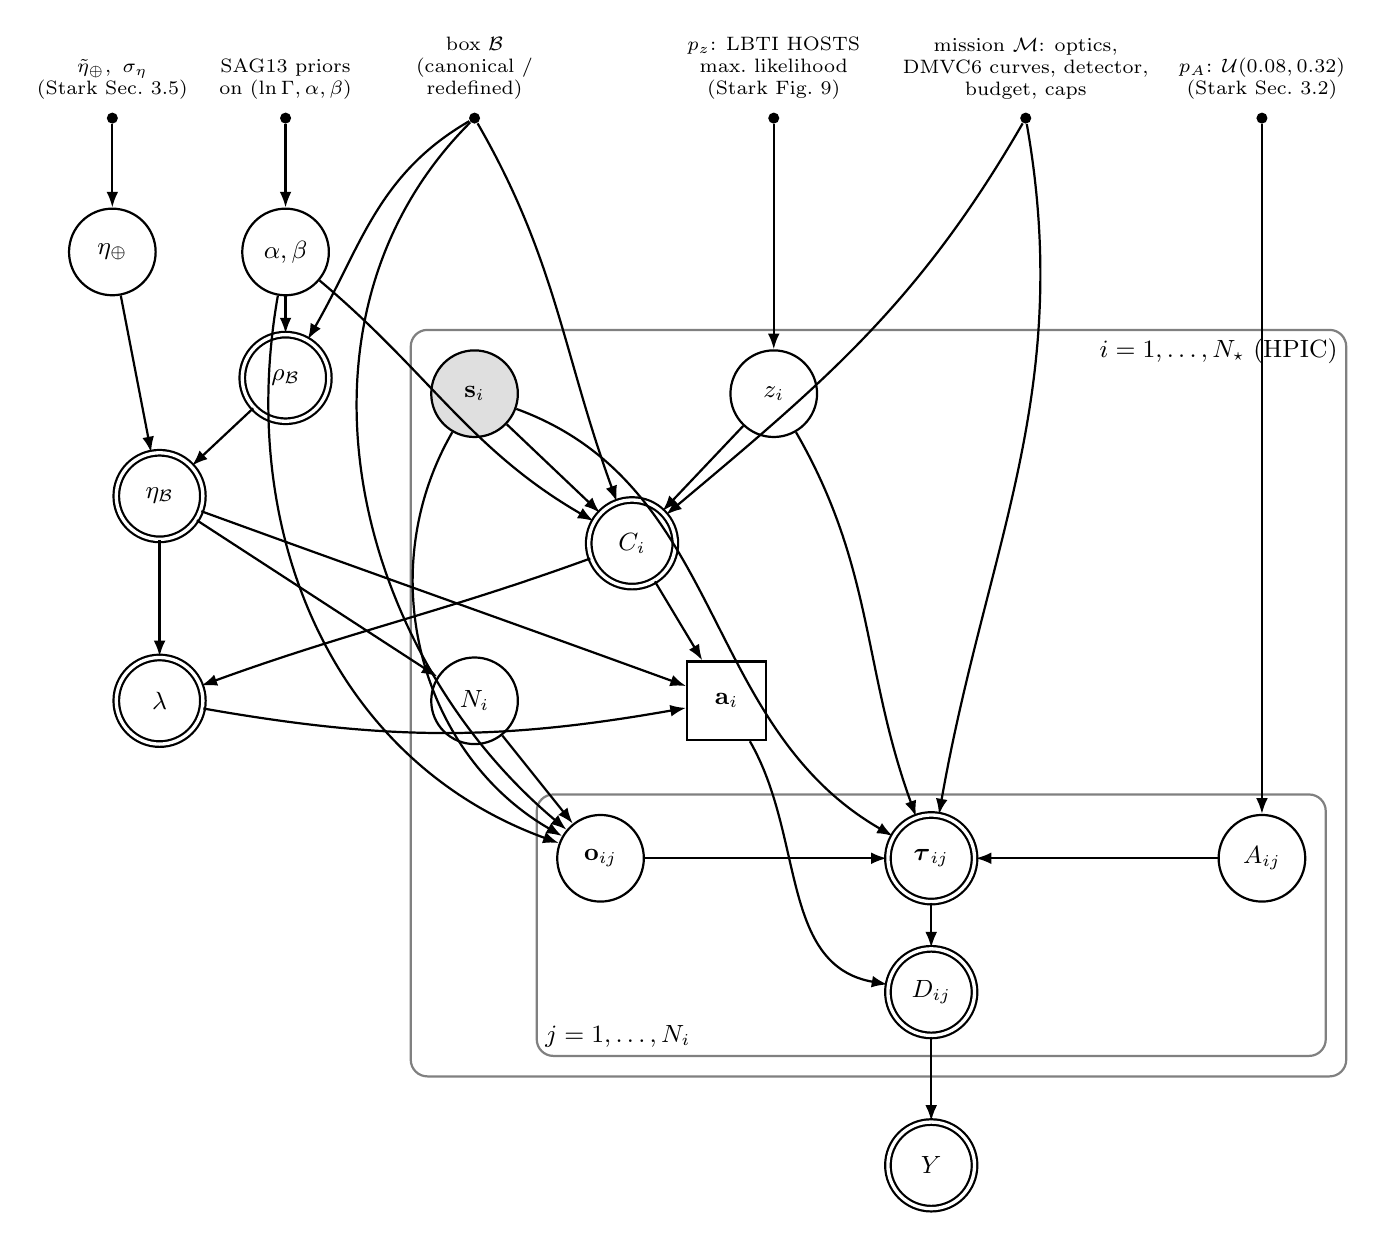
\begin{tikzpicture}[x=1cm,y=1cm]
  % ---- global hyperparameters (fixed) ----
  \node[fixed] (hEta) at (0,0) {};
  \node[flabel,above=1pt of hEta] {$\tilde\eta_\oplus,\ \sigma_\eta$\\(Stark Sec.~3.5)};
  \node[fixed] (hShape) at (2.2,0) {};
  \node[flabel,above=1pt of hShape] {SAG13 priors\\on $(\ln\Gamma,\alpha,\beta)$};
  \node[fixed] (hBox) at (4.6,0) {};
  \node[flabel,above=1pt of hBox] {box $\mathcal{B}$\\(canonical /\\redefined)};
  \node[fixed] (hZ) at (8.4,0) {};
  \node[flabel,above=1pt of hZ] {$p_z$: LBTI HOSTS\\max.\ likelihood\\(Stark Fig.~9)};
  \node[fixed] (hM) at (11.6,0) {};
  \node[flabel,above=1pt of hM] {mission $\mathcal{M}$: optics,\\DMVC6 curves, detector,\\budget, caps};
  \node[fixed] (hA) at (14.6,0) {};
  \node[flabel,above=1pt of hA] {$p_A$: $\mathcal{U}(0.08,0.32)$\\(Stark Sec.~3.2)};
  % ---- global latent / deterministic ----
  \node[latent] (eta) at (0,-1.7) {$\eta_\oplus$};
  \node[latent] (shape) at (2.2,-1.7) {$\alpha,\beta$};
  \node[det] (rho) at (2.2,-3.3) {$\rho_{\mathcal{B}}$};
  \node[det] (etaB) at (0.6,-4.8) {$\eta_{\mathcal{B}}$};
  \node[det] (lambda) at (0.6,-7.4) {$\lambda$};
  % ---- star plate ----
  \node[obs] (s) at (4.6,-3.5) {$\mathbf{s}_i$};
  \node[latent] (z) at (8.4,-3.5) {$z_i$};
  \node[det] (C) at (6.6,-5.4) {$C_i$};
  \node[latent] (N) at (4.6,-7.4) {$N_i$};
  \node[dec] (a) at (7.8,-7.4) {$\mathbf{a}_i$};
  % ---- planet plate ----
  \node[latent] (o) at (6.2,-9.4) {$\mathbf{o}_{ij}$};
  \node[det] (tau) at (10.4,-9.4) {$\boldsymbol{\tau}_{ij}$};
  \node[latent] (A) at (14.6,-9.4) {$A_{ij}$};
  \node[det] (D) at (10.4,-11.1) {$D_{ij}$};
  % ---- yield ----
  \node[det] (Y) at (10.4,-13.3) {$Y$};
  \coordinate (Aright) at (15.4,-9.4);
  % ---- plates ----
  \begin{scope}[on background layer]
    \node[plate,fit=(o) (tau) (A) (D)] (pp) {};
    \node[plate,fit=(s) (z) (C) (N) (a) (pp) (Aright)] (sp) {};
  \end{scope}
  \node[font=\small,anchor=south west] at (pp.south west) {$j = 1,\dots,N_i$};
  \node[font=\small,anchor=north east] at (sp.north east) {$i = 1,\dots,N_\star$ (HPIC)};
  % ---- edges ----
  \draw[edge] (hEta) -- (eta);
  \draw[edge] (hShape) -- (shape);
  \draw[edge] (shape) -- (rho);
  \draw[edge] (hBox) to[out=-150,in=60] (rho);
  \draw[edge] (eta) -- (etaB);
  \draw[edge] (rho) -- (etaB);
  \draw[edge] (etaB) -- (lambda);
  \draw[edge] (etaB) to[out=-20,in=160] (a);
  \draw[edge] (etaB) -- (N);
  \draw[edge] (C) to[out=-160,in=20] (lambda);
  \draw[edge] (lambda) to[out=-10,in=-170] (a);
  \draw[edge] (C) -- (a);
  \draw[edge] (hZ) -- (z);
  \draw[edge] (s) -- (C);
  \draw[edge] (z) -- (C);
  \draw[edge] (hBox) to[out=-135,in=140] (o);
  \draw[edge] (s) to[out=-20,in=150] (tau);
  \draw[edge] (hBox) to[out=-60,in=110] (C);
  \draw[edge] (shape) to[out=-40,in=150] (C);
  \draw[edge] (hM) to[out=-120,in=40] (C);
  \draw[edge] (s) to[out=-120,in=150] (o);
  \draw[edge] (shape) to[out=-100,in=160] (o);
  \draw[edge] (N) -- (o);
  \draw[edge] (o) -- (tau);
  \draw[edge] (A) -- (tau);
  \draw[edge] (hA) -- (A);
  \draw[edge] (z) to[out=-60,in=110] (tau);
  \draw[edge] (hM) to[out=-80,in=80] (tau);
  \draw[edge] (tau) -- (D);
  \draw[edge] (a) to[out=-60,in=170] (D);
  \draw[edge] (D) -- (Y);
\end{tikzpicture}}

\vspace{0.6em}
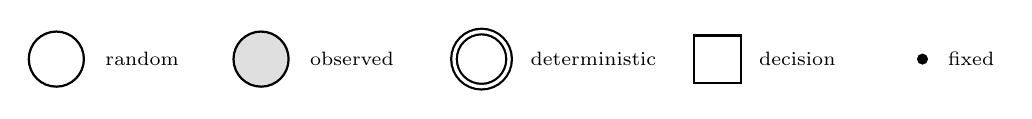
\begin{tikzpicture}[x=1cm,y=1cm]
  \node[latent,minimum size=7mm] at (0,0) {}; \node[font=\scriptsize,anchor=west] at (0.5,0) {random};
  \node[obs,minimum size=7mm] at (2.6,0) {}; \node[font=\scriptsize,anchor=west] at (3.1,0) {observed};
  \node[det,minimum size=7mm] at (5.4,0) {}; \node[font=\scriptsize,anchor=west] at (5.9,0) {deterministic};
  \node[dec,minimum size=6mm] at (8.4,0) {}; \node[font=\scriptsize,anchor=west] at (8.8,0) {decision};
  \node[fixed] at (11.0,0) {}; \node[font=\scriptsize,anchor=west] at (11.2,0) {fixed};
\end{tikzpicture}
\caption{The yield model as an influence diagram. Outer plate: the $N_\star$ screened HPIC stars;
inner plate: the $N_i$ planets actually present around star $i$. The survey allocation
$\mathbf{a}_i = (\tau_i, k_i)$ --- exposure per visit and number of visits --- is the one decision
node; it is set by the equal-slope multiplier $\lambda$ from the planner's completeness curves
$C_i$ and the box occurrence rate $\eta_{\mathcal{B}}$. A planet is counted ($D_{ij} = 1$) when
its detection time at some visit is within the allocation and its spectral characterization time
is within the two-month cap; $Y = \sum_{ij} D_{ij}$. Four stars with LBTI-measured exozodi have
$z_i$ observed rather than drawn (not shown).
The edges that decide the uncertainty budget are the ones \emph{into} $\mathbf{a}_i$: $\eta_\oplus$
and $z_i$ reach it (actionable), $A_{ij}$ and $N_i$ do not (static).}
\label{fig:pgm}
\end{figure}

\subsection{The nodes}

\begin{table}[htbp]
\centering
\scriptsize
\begin{tabular}{p{1.2cm}p{3.2cm}p{5.6cm}p{3.6cm}}
\toprule
\textbf{Node} & \textbf{Type} & \textbf{Specification} & \textbf{Source; step} \\
\midrule
$\eta_\oplus$ & random, global & lognormal, median 0.257, $\ln$-width 0.76 (Sec.~\ref{sec:eta}) & Stark+2024 Sec.~3.5, read at $z=1$; A06 \\
$\alpha,\beta$ & random, global & SAG13 shape; posterior of an \texttt{emcee} chain, used only through $\rho_\mathcal{B}$ & SAG13; A06 \\
$\rho_\mathcal{B}$ & deterministic & $\eta_\mathcal{B}/\eta_\oplus$, the SAG13 integral over $\mathcal{B}$ relative to the canonical box; independent of $\Gamma$ & A06 \\
$\eta_\mathcal{B}$ & deterministic & $\eta_\oplus\,\rho_\mathcal{B}$ & A06 \\
$\mathbf{s}_i$ & observed & $d$, $L_\star$, $T_{\rm eff}$, $R_\star$, HIP id & HPIC (Tuchow+2024); A01 \\
$z_i$ & random, per star & exozodi level, $z_i \sim p_z$; four stars fixed at LBTI values; 200 joint draws of $\mathbf{z}$ & Stark+2024 Sec.~3.3, Fig.~9; A02, A04 \\
$C_i$ & deterministic & planner's completeness $C_i(\tau, k)$ at $A_G = 0.2$, over exposure and visits, counting only planets that are also characterizable & Stark+2019; A04 \\
$\lambda$ & deterministic & equal-slope multiplier closing the two-year budget & Stark+2014; A05 \\
$\mathbf{a}_i$ & decision & $(\tau_i, k_i)$: the vertex of star $i$'s concave cost envelope at slope $\lambda$ & A05, A07 \\
$N_i$ & random, per star & $N_i \sim \mathrm{Poisson}(\eta_\mathcal{B})$ & Stark+2024 Sec.~3.1; A07 \\
$\mathbf{o}_{ij}$ & random, per planet & circular orbit: $a$, $R$ from SAG13 over $\mathcal{B}$; $\cos i \sim \mathcal{U}$; independent epoch per visit & ExoVista/AYO; A04 \\
$A_{ij}$ & random, per planet & geometric albedo, $\mathcal{U}(0.08, 0.32)$, counted by Stark's per-visit flux test & Stark+2024 Sec.~3.2; A02, A04 \\
$\boldsymbol{\tau}_{ij}$ & deterministic & detection time per visit (two channels in quadrature, S/N 7) and characterization time (R 140, best of nine bandpasses, best orbital phase) & Stark+2019 Eqs.~1--9; A04 \\
$D_{ij}$ & deterministic & $\mathbb{1}[\min_{v \le k_i}\tau^{\rm det}_{ijv} \le \tau_i \ \wedge\ \tau^{\rm char}_{ij} \le 2\,\mathrm{mo}]$ & Stark+2019 Sec.~3; A04 \\
$Y$ & deterministic & $\sum_{i,j} D_{ij}$ & A07 \\
\bottomrule
\end{tabular}
\caption{Every node of Fig.~\ref{fig:pgm}, what it is, and where it comes from.}
\label{tab:nodes}
\end{table}

\subsection{What we do not calibrate}
\label{sec:kappa}

A common way to absorb the unpublished parts of a model is a scalar throughput factor $\kappa$
on every band, fitted so that the canonical box reproduces the published 22.5 candidates. We do
not use one, for two reasons. First, no Stark paper contains such a factor: 22.5 is an output of
AYO, not an input to it, so a reproduction that fits to it is not reproducing the same quantity.
Second, a fitted factor hides errors. We measured the effect of every alternative treatment we
tested on the per-planet exposure times, and found that with $\kappa$ refitted each of them
changes those times by a nearly uniform factor of $1.0 \pm 0.05$. Because the yield responds to
throughput with an elasticity of only $\sim0.4$, a fitted factor can absorb any such change
completely, and a whole class of modeling errors becomes invisible. Without it, the two residues of
Secs.~\ref{sec:char} and~\ref{sec:eta} are visible as residues rather than silently rescaled
away. For reference, the factor that would reproduce 22.5 is 1.20.

One sourced term matters a great deal here: the extended-source throughput $T_{\rm sky}$ that
Stark et al.\ (2019) Eqs.~5--6 apply to the zodiacal and exozodiacal backgrounds. Its radial
shape is not published, so the reconstruction is ours, and it very probably differs from AYO's
near the inner working angle. Section~\ref{sec:tsky} gives our reconstruction, what AYO's is
likely to be, and by how much they differ.

%======================================================================
\section{The model in equations}
\label{sec:equations}
%======================================================================

This section states every equation the pipeline evaluates, in the order it evaluates them, with
each variable defined where it first appears. Table~\ref{tab:params} lists the scalar parameters
with their values and sources, and Table~\ref{tab:bands} the detection channels and spectral
bandpasses. Throughout, $D$ is the inscribed diameter by which Stark et al.\ (2024) label the
design, and $D_{\rm circ} = 7.16$\,m the circumscribed diameter against which the published
coronagraph curves are plotted.

\begin{table}[htbp]
\centering
\scriptsize
\begin{tabular}{p{8.2cm}rp{3.6cm}}
\toprule
\textbf{Parameter} & \textbf{Value} & \textbf{Source} \\
\midrule
Inscribed diameter $D$ (m) & 6.0 & S24 \\
Circumscribed / inscribed diameter & 1.194 & LUVOIR-B, 8\,m / 6.7\,m \\
Area fill factor $f_{\rm fill}$ & 0.785 & none published \\
Contamination throughput $\tau_{\rm con}$ & 0.95 & S24 \\
Quantum efficiency $Q$ & 0.90 & S24 \\
Detective quantum efficiency $q$ & 0.75 & S24 \\
Dark current $\xi_{\rm DC}$ (counts\,pix$^{-1}$\,s$^{-1}$) & $3.0\times10^{-5}$ & S24 \\
Read noise (counts\,pix$^{-1}$) & 0 & S24 (photon counting) \\
Clock-induced charge $\xi_{\rm CIC}$ (counts\,pix$^{-1}$\,frame$^{-1}$) & $1.3\times10^{-3}$ & S24 \\
Raw-contrast floor $\zeta_{\rm floor}$ & $10^{-10}$ & S19 \\
Photometric aperture radius $X$ ($\lambda/D$) & 0.7 & S19 \\
Noise floor $\Delta m_{\rm nf}$ (mag) & 26.5 & S24 \\
Planning albedo $A_{\rm plan}$ & 0.20 & S24 Sec.~3.2 \\
Exozodi surface brightness per zodi at $V$ (mag\,arcsec$^{-2}$) & 22.0 & S14 \\
Survey time $T$ (yr) & 2.0 & S24 \\
Exposure limit $t_{\rm lim}$, including overheads (d) & 60 & S24 \\
Slew overhead $t_{\rm slew}$ (h) & 1.0 & S24 \\
Wavefront-control overhead $t_{\rm WFC}$ (h) & 2.7 & S24 \\
Wavefront-control time multiplier $\tau'$ & 1.10 & S24 \\
Maximum visits per star $k_{\max}$ & 6 & S15 \\
\midrule
Circumscribed diameter $D_{\rm circ}$ (m) & 7.16 & derived \\
Collecting area $A = f_{\rm fill}\,\pi D_{\rm circ}^2/4$ (m$^2$) & 31.6 & derived \\
Longest science exposure $\tau_{\rm cap}$ (d), Eq.~\eqref{eq:cap} & 54.4 & derived \\
Airy encircled energy in the aperture, ${\rm EE}(X)$ & 0.678 & derived \\
Peak DMVC6 core throughput $\Upsilon_{c,\max}$ & 0.388 & digitized \\
\bottomrule
\end{tabular}
\caption{Scalar parameters of the baseline mission. S14, S15, S19 and S24 are Stark et al.\
(2014, 2015, 2019, 2024); S24 values are from its Tables~1 and~2 unless a section is given. The
DMVC6 core throughput $\Upsilon_c(r)$ and raw contrast $\zeta(r)$ are digitized from Stark et al.\
(2024) and shown in Fig.~\ref{fig:pair25}.}
\label{tab:params}
\end{table}

\begin{table}[htbp]
\centering
\small
\begin{tabular}{llrrrrr}
\toprule
\textbf{Name} & \textbf{Use} & $\lambda$ \textbf{(nm)} & $\Delta\lambda/\lambda$ & $\tau_b$ &
\textbf{S/N} & $N_{\rm pix}$ \\
\midrule
LW & detection & 550 & 0.20 & 0.34 & 7 & 4 \\
SW & detection & 450 & 0.20 & 0.15 & 7 & 4 \\
IFS730 & spectrum & 730 & 1/140 & 0.23 & 17 & 51 \\
IFS763 & spectrum & 763 & 1/140 & 0.23 & 15 & 56 \\
IFS779 & spectrum & 779 & 1/140 & 0.23 & 14 & 58 \\
IFS824 & spectrum & 824 & 1/140 & 0.23 & 13 & 65 \\
IFS842 & spectrum & 842 & 1/140 & 0.23 & 12 & 68 \\
IFS917 & spectrum & 917 & 1/140 & 0.23 & 10 & 81 \\
IFS930 & spectrum & 930 & 1/140 & 0.23 & 9 & 83 \\
IFS943 & spectrum & 943 & 1/140 & 0.23 & 6 & 85 \\
IFS1000 & spectrum & 1000 & 1/140 & 0.23 & 5 & 96 \\
\bottomrule
\end{tabular}
\caption{Detection channels and characterization bandpasses. $\tau_b$ is the optical throughput
of the channel, S/N the required signal-to-noise ratio (per spectral bin for the spectra), and
$N_{\rm pix}$ the number of detector pixels the signal is spread over. The two detection channels
observe in parallel and their S/N adds in quadrature; a spectrum uses whichever single bandpass
is fastest. The spectral bandpasses and their S/N follow Stark et al.\ (2024) Fig.~3.}
\label{tab:bands}
\end{table}

\subsection{Stars}

Star $i$ has distance $d_i$, luminosity $L_i$, effective temperature $T_i$, radius $R_{\star,i}$
and ecliptic latitude $b_i$, all from HPIC. Its photon spectral flux at the telescope is a
blackbody,
\begin{equation}
F_\star(\lambda) = \pi\left(\frac{R_\star}{d}\right)^{2} B_\lambda(T)\,\frac{\lambda}{hc}
\qquad [\mathrm{photons\ s^{-1}\,m^{-2}\,m^{-1}}],
\label{eq:starflux}
\end{equation}
where $B_\lambda$ is the Planck function. Its Earth-equivalent insolation distance is
$a_{\rm EEID} = \sqrt{L/L_\odot}$\,AU.

\subsection{Occurrence and the selection boxes}

Planets follow the SAG13 density
\begin{equation}
\frac{d^2N}{d\ln R\,d\ln P} = \Gamma\,R^{\alpha}P^{\beta},
\label{eq:sag13}
\end{equation}
with $R$ in Earth radii and $P$ in years. A selection box $\mathcal{B}$ is a range of scaled
semi-major axis $a' = a/a_{\rm EEID} \in [a'_{\rm in}, a'_{\rm out}]$ and a radius range
$[R_{\rm lo}(a'), R_{\rm hi}]$. Since $P \propto a^{3/2}$ at the solar-twin reference, the
occurrence over the box is
\begin{equation}
\eta_\mathcal{B} = \frac{3}{2}\,\Gamma\int_{a'_{\rm in}}^{a'_{\rm out}} a'^{\,3\beta/2}
\int_{R_{\rm lo}(a')}^{R_{\rm hi}} R^{\alpha}\,d\ln R\;d\ln a'.
\label{eq:etabox}
\end{equation}
The canonical box has $a' \in [0.95, 1.67]$, $R_{\rm lo} = 0.8\,a'^{-1/2}$ and $R_{\rm hi} = 1.4$.
The redefined box has $a' \in [0.96, 1.20]$ and $0.5 \le M/M_\oplus \le 2$ with $R = M^{0.27}$,
i.e.\ $R \in [0.829, 1.206]$. The ratio $\rho_\mathcal{B} = \eta_\mathcal{B}/\eta_{\rm canon}$
does not depend on $\Gamma$; it is computed over an \texttt{emcee} chain in
$(\ln\Gamma, \alpha, \beta)$ with SAG13 priors $\alpha = -0.19 \pm 0.27$ and
$\beta = 0.26 \pm 0.29$.

The canonical occurrence $\eta_\oplus \equiv \eta_{\rm canon}$ is lognormal,
\begin{equation}
\ln\eta_\oplus \sim \mathcal{N}(\mu, \sigma^2), \qquad
\mu = \tfrac{1}{2}\ln(\eta_{\rm lo}\,\eta_{\rm hi}), \qquad
\sigma = \frac{\ln(\eta_{\rm hi}/\eta_{\rm lo})}{2z},
\label{eq:etalaw}
\end{equation}
where $[\eta_{\rm lo}, \eta_{\rm hi}] = [0.12, 0.55]$ is the interval quoted by Stark et al.\
(2024) and $z$ is the number of standard deviations it is taken to span. We adopt $z = 1$
(a 68\% interval), which gives a median $e^{\mu} = 0.257$, $\sigma = 0.76$ and a mean of
0.343; Sec.~\ref{sec:eta} explains and tests this choice. The redefined box then has
$\eta_\mathcal{B} = \rho_\mathcal{B}\,\eta_\oplus$.

\subsection{Injected planets and their geometry}

For each star and box, $N_{\rm inj}$ = 1\,200--3\,000 planets are drawn: $a'$ from a density
$\propto a'^{\,3\beta/2}\,d\ln a'$ on the box's range, $R$ from $\propto R^{\alpha}\,d\ln R$ on
its radius range (with $\alpha$ and $\beta$ at their SAG13 central values), $\cos i$ uniform on
$[-1, 1]$, and, for each of up to $k_{\max}$ visits $v$, an independent orbital angle $\theta_v$
uniform on $[0, 2\pi)$. Orbits are circular with radius $a = a'\,a_{\rm EEID}$. At visit $v$ the
projected separation and phase angle $\phi$ are
\begin{equation}
s_v = a\sqrt{\cos^2\theta_v + \sin^2\theta_v\cos^2 i}, \qquad
\cos\phi_v = \sin\theta_v\,\sin i,
\label{eq:geometry}
\end{equation}
and the planet-to-star flux ratio is
\begin{equation}
f_v = A\,\Phi(\phi_v)\left(\frac{R_p}{a}\right)^{2}, \qquad
\Phi(\phi) = \frac{\sin\phi + (\pi - \phi)\cos\phi}{\pi},
\label{eq:fluxratio}
\end{equation}
with $A$ the geometric albedo: $A_{\rm plan} = 0.2$ for planning and a draw from
$\mathcal{U}(0.08, 0.32)$ for counting (Sec.~\ref{sec:counting}). The separation in the units of
the coronagraph curves is
\begin{equation}
r_v = \frac{s_v/d}{\lambda/D}\cdot\frac{D_{\rm circ}}{D},
\label{eq:separation}
\end{equation}
with $s_v/d$ in radians.

\subsection{Count rates}

For a channel $b$ with central wavelength $\lambda$, bandwidth $\Delta\lambda$, optical throughput
$\tau_b$ and $N_{\rm pix}$ pixels, the end-to-end throughput is
$\tau = \tau_b\,\tau_{\rm con}\,Q\,q$ and the stellar count rate is
$\mathrm{CR}_\star = F_\star(\lambda)\,\Delta\lambda\,A_{\rm tel}\,\tau$, where
$A_{\rm tel} = 31.6$\,m$^2$ is the collecting area (Table~\ref{tab:params}). The coronagraph
enters through the core throughput $\Upsilon_c(r)$ and the raw contrast
$\zeta(r) = \max[\zeta_{\rm DMVC6}(r), \zeta_{\rm floor}]$. With
$\Omega = \pi(X\lambda/D)^2$ the solid angle of the photometric aperture of radius $X$, the
count rates are
\begin{align}
\mathrm{CR}_p &= \mathrm{CR}_\star\,\Upsilon_c(r)\,f, \label{eq:crp}\\
\mathrm{CR}_{\rm leak} &= \mathrm{CR}_\star\,\Upsilon_c(r)\,\zeta(r), \label{eq:crleak}\\
\mathrm{CR}_z &= I_z\,\Delta\lambda\;\Omega\,A_{\rm tel}\,\tau\;T_{\rm sky}(r), \label{eq:crz}\\
\mathrm{CR}_{ez} &= z\,I_{ez}\,\Delta\lambda\;\Omega\,A_{\rm tel}\,\tau\;T_{\rm sky}(r),
\label{eq:crez}\\
\mathrm{CR}_{\rm det} &= N_{\rm pix}\left[\xi_{\rm DC} + 6.73\,\xi_{\rm CIC}\,
\frac{\mathrm{CR}_p + \mathrm{CR}_{\rm leak} + \mathrm{CR}_z + \mathrm{CR}_{ez}}{N_{\rm pix}}
\right]. \label{eq:crdet}
\end{align}
Here $I_z$ is the local zodiacal surface brightness,
$I_z = 0.69\,I_{90}(\lambda)\,f_{135}(b)$, with $I_{90}$ the Leinert et al.\ (1998) spectrum at
$90^\circ$ elongation and $f_{135}(b) = 1.02 - 0.566x - 0.884x^2 + 0.853x^3$, $x = |\sin b|$
(Stark et al.\ 2014); $z$ is the star's exozodi level in zodis; and
\begin{equation}
I_{ez} = F_0(\lambda)\,10^{-0.4\times 22}\;
\frac{F_\star(\lambda)|_{10\,{\rm pc}}}{F_\odot(\lambda)|_{10\,{\rm pc}}}\;\frac{L_\odot}{L}
\label{eq:iez}
\end{equation}
is the surface brightness of one zodi of exozodiacal dust around that star, held at constant
habitable-zone optical depth (Stark et al.\ 2014, App.~C). $F_0(\lambda)$ is a solar-colored
zero point normalized to $10^{11}$ photons\,s$^{-1}$\,m$^{-2}$\,$\mu$m$^{-1}$ at $V$. The
detector term is Stark et al.\ (2019) Eq.~9: dark current plus clock-induced charge, whose frame
rate is set by the brightest pixel, with the Geiger factor 6.73. The total background is
$\mathrm{CR}_b = \mathrm{CR}_{\rm leak} + \mathrm{CR}_z + \mathrm{CR}_{ez} + \mathrm{CR}_{\rm det}$.

\subsection{The extended-source throughput $T_{\rm sky}$}
\label{sec:tsky}

Only the two sky terms, Eqs.~\eqref{eq:crz} and~\eqref{eq:crez}, carry $T_{\rm sky}$. Stark et
al.\ (2019, Eqs.~5--6) define it as ``the instrument's throughput for extended sources'',
computed ``by first convolving the spatially-dependent PSF at all locations with a normalized
uniform background''. For a uniform background, the light an aperture at $r$ collects is the sum,
over every point of the sky nearby, of the fraction of that point's light the coronagraph
delivers into the aperture. $T_{\rm sky}(r)$ therefore counts \emph{all} transmitted light
landing in the aperture, from the cores and the wings of the PSFs of every nearby point, while
$\Upsilon_c(r)$ counts only the core of one point source. Stark's DMVC6 map is not published, so
it has to be reconstructed.

\textbf{Our reconstruction.} Write $\Upsilon_c(r) = T_{\rm tot}(r)\,\epsilon_{\rm core}(r)$, the
total fraction $T_{\rm tot}$ of an off-axis source's light that the coronagraph transmits times
the fraction $\epsilon_{\rm core}$ of that light falling inside the photometric aperture. If the
off-axis PSF keeps the Airy shape at every separation, $\epsilon_{\rm core} = {\rm EE}(X)$, and if
$T_{\rm tot}$ changes little across one $\lambda/D$, the convolution returns $T_{\rm tot}$ itself.
Under those two assumptions
\begin{equation}
T_{\rm sky}(r) = \frac{\Upsilon_c(r)}{{\rm EE}(X)} = 1.474\,\Upsilon_c(r),
\label{eq:tsky}
\end{equation}
since ${\rm EE}(0.7) = 0.678$. For the DMVC6, $T_{\rm sky}$ therefore rises from 0.08 at
$2\,\lambda/D$ to 0.572 at the outer edge of the dark hole, in exact proportion to the core
throughput (Table~\ref{tab:tsky}, Fig.~\ref{fig:tsky}).

\textbf{What AYO probably does.} AYO computes the convolution from its simulated two-dimensional
off-axis PSFs, and both of our assumptions fail near the inner working angle. There the
focal-plane mask distorts the off-axis PSF and moves light from its core into its wings, so
$\epsilon_{\rm core}$ falls below ${\rm EE}(X)$; and the convolution averages $T_{\rm tot}$ over
about one $\lambda/D$, pulling in light from larger separations where more is transmitted. Both
raise $T_{\rm sky}/\Upsilon_c$ toward the inner working angle, where Eq.~\eqref{eq:tsky} holds it
constant. The only AYO values in print are for a different coronagraph, the vortex of the Stark
et al.\ (2025) exposure-time benchmark. There AYO's $T_{\rm sky}/\Upsilon_c$ rises from
1.8 at 5.7\,$\lambda/D$ to 3.2 at 2.1\,$\lambda/D$, and
Eq.~\eqref{eq:tsky} applied to that coronagraph gives only 0.47--0.81 of
AYO's value. We condense the benchmark into a correction factor linear in the core fraction
$u = \Upsilon_c/\Upsilon_{c,\max}$,
\begin{equation}
T_{\rm sky}^{\rm AYO\text{-}like}(r) = T_{\rm sky}(r)\,\big[F_0 + (F_1 - F_0)\,u\big],
\qquad F_0 = 2.19,\quad F_1 = 1.08,
\label{eq:tskyayo}
\end{equation}
which fits the benchmark to 6\% rms. Applied to the DMVC6, this AYO-like shape exceeds
ours by a factor of 2.04 at $2\,\lambda/D$, 1.52 at $5\,\lambda/D$ and 1.26 at
$10\,\lambda/D$ (Table~\ref{tab:tsky}).

\begin{table}[htbp]
\centering
\small
\begin{tabular}{rrrrr}
\toprule
$r$ ($\lambda/D_{\rm circ}$) & $\Upsilon_c$ & $T_{\rm sky}$, Eq.~\eqref{eq:tsky} &
$T_{\rm sky}$, AYO-like & \textbf{ratio} \\
\midrule
1.5 & 0.016 & 0.023 & 0.050 & 2.15 \\
2.0 & 0.053 & 0.079 & 0.160 & 2.04 \\
2.5 & 0.097 & 0.143 & 0.274 & 1.91 \\
3.0 & 0.134 & 0.197 & 0.357 & 1.81 \\
3.5 & 0.168 & 0.247 & 0.423 & 1.71 \\
4.0 & 0.195 & 0.288 & 0.470 & 1.63 \\
5.0 & 0.235 & 0.347 & 0.527 & 1.52 \\
7.0 & 0.286 & 0.421 & 0.579 & 1.38 \\
10.0 & 0.325 & 0.480 & 0.605 & 1.26 \\
15.0 & 0.357 & 0.527 & 0.616 & 1.17 \\
20.0 & 0.373 & 0.550 & 0.619 & 1.12 \\
25.0 & 0.382 & 0.564 & 0.619 & 1.10 \\
\bottomrule
\end{tabular}
\caption{The DMVC6 core throughput and the two reconstructions of its extended-source throughput.
The last column is the AYO-like value divided by ours.}
\label{tab:tsky}
\end{table}

\begin{figure}[htbp]
\centering
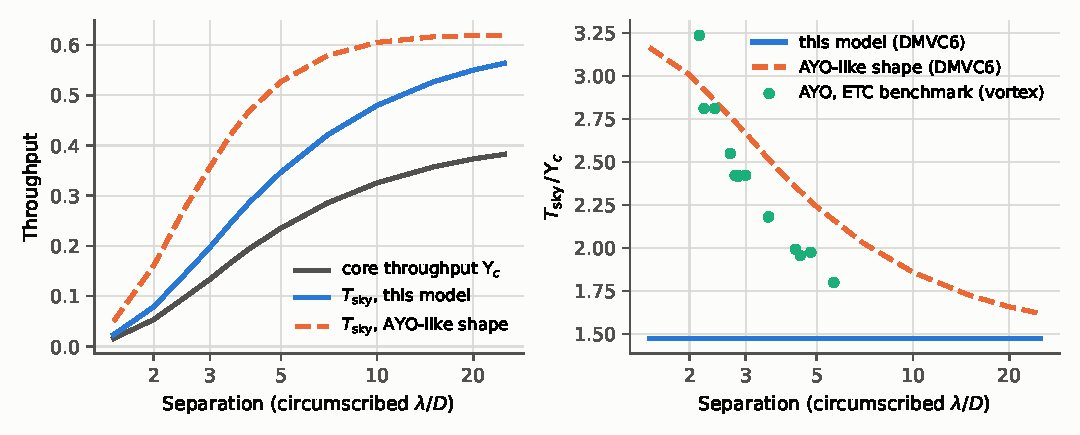
\includegraphics[width=\textwidth]{figSkyThroughputShapes.pdf}
\caption{Left: DMVC6 core throughput and the two reconstructions of $T_{\rm sky}$. Right: their
ratio to the core throughput. Ours (Eq.~\eqref{eq:tsky}) is constant at 1.474; the
AYO-like shape (Eq.~\eqref{eq:tskyayo}) rises toward the inner working angle, following AYO's own
values for the vortex coronagraph of the Stark et al.\ (2025) benchmark (points).}
\label{fig:tsky}
\end{figure}

\textbf{Why this could matter, and what it does.} $T_{\rm sky}$ multiplies the zodiacal and
exozodiacal backgrounds, and at $R = 140$ near $1\,\mu$m the exozodiacal term dominates the noise
of a spectrum. The planets that sit closest to the inner working angle are those around distant
and luminous stars, which are exactly the targets on which our survey and Stark's disagree
(Sec.~\ref{sec:char}). A larger $T_{\rm sky}$ near the inner working angle is therefore a natural
candidate for the characterization-time discrepancy, and the term demonstrably matters for the
absolute yield: holding $T_{\rm sky}$ at its large-separation value lowers the mean realized yield
from 22.4 to 19.2 (Table~\ref{tab:variants}). We test the AYO-like shape
directly in Sec.~\ref{sec:char}, as one of the four parameters of the throughput study, and find
that it moves the model along the same curve as every other throughput change rather than toward
Stark's published values (Fig.~\ref{fig:degobs}). A DMVC6 map that departs from ours by more than
the vortex benchmark suggests cannot be excluded, and it is part of Question~1
(Sec.~\ref{sec:discussion}).

\subsection{Exposure times}

For each channel $c$ define
\[
a_c = \mathrm{CR}_{p,c}^2, \qquad v_c = \mathrm{CR}_{p,c} + 2\,\mathrm{CR}_{b,c}, \qquad
n_c = \zeta_{\rm nf}\,\mathrm{CR}_{\star,c}\,\Upsilon_c(r), \qquad
\zeta_{\rm nf} = \frac{10^{-0.4\,\Delta m_{\rm nf}}\sqrt{N_{\rm ch}}}{({\rm S/N})_d},
\]
where $n_c$ is the noise-floor rate and $\zeta_{\rm nf}$ the contrast that reaches the detection S/N only in infinite time with all $N_{\rm ch} = 2$
channels combined. The
exposure time $t$ that reaches signal-to-noise ${\rm S/N}$ solves
\begin{equation}
\sum_c \frac{a_c\,t}{v_c + n_c^2\,t} = ({\rm S/N})^2,
\label{eq:exptime}
\end{equation}
which for a single channel is
$t = ({\rm S/N})^2\,v/[a - ({\rm S/N})^2 n^2]$, Stark et al.\ (2025) Eq.~1, and without the
floor ($n = 0$) reduces to Stark et al.\ (2019) Eq.~1. A planet with
$\sum_c a_c/n_c^2 \le ({\rm S/N})^2$ can never be detected, and $t = \infty$. Detection uses the
two channels of Table~\ref{tab:bands} at ${\rm S/N} = 7$, giving $t^{\rm det}_{jv}$ for planet $j$
at visit $v$. A spectrum uses one bandpass $o$ at its own S/N; its time is minimized over the
bandpasses and over 40 orbital angles $\theta$, because the orbit is known by the time a spectrum
is taken (Stark et al.\ 2019):
\begin{equation}
t^{\rm char}_j = \min_{o,\,\theta}\,t_o(\theta).
\label{eq:tchar}
\end{equation}
The two-month limit applies to the exposure including overheads, so the longest science exposure
is
\begin{equation}
\tau_{\rm cap} = \frac{t_{\rm lim} - t_{\rm slew} - t_{\rm WFC}}{\tau'} = 54.4\ {\rm d}.
\label{eq:cap}
\end{equation}

\subsection{Counting, completeness and the albedo test}
\label{sec:counting}

At planning albedo, planet $j$ counts for a star observed $k$ times with exposure $t$ per visit if
it is detected on at least one of those visits and its spectrum fits under the cap:
\begin{equation}
D_j(t, k) = \mathbb{1}\Big[\min_{v \le k} t^{\rm det}_{jv} \le \min(t, \tau_{\rm cap})\ \wedge\
t^{\rm char}_j \le \tau_{\rm cap}\Big],
\label{eq:counted}
\end{equation}
and the star's completeness is the counted fraction,
$C(t, k) = N_{\rm inj}^{-1}\sum_j D_j(t, k)$. The mean characterization time of the counted
planets, $\bar t_{\rm char}(t, k)$, is what the survey budgets for spectra.

To count planets with drawn albedos we follow Stark et al.\ (2024) Sec.~3.2: the plan stays fixed
at $A_{\rm plan}$, and a planet with drawn albedo $A_j$ is counted at visit $v$ only if the fixed
plan would have caught it. Let $\mathcal{S}_v(t)$ be the set of planning-albedo planets detected
at visit $v$ within exposure $t$. The drawn planet passes at the smallest $t$ for which its flux
$f_{jv}A_j/A_{\rm plan}$ is at least the faintest flux in $\mathcal{S}_v(t)$ and its separation is
at least the smallest separation in $\mathcal{S}_v(t)$, and it fails outright if its flux exceeds
the brightest flux any detectable planet reaches, which the inner working angle bounds. Replacing
$t^{\rm det}_{jv}$ in Eq.~\eqref{eq:counted} by that threshold gives the completeness actually
realized, $\bar C(t, k)$. Spectra are budgeted at $A_{\rm plan}$, as Stark states.

\subsection{The survey allocation}

Visiting star $i$ $k$ times with exposure $t$ costs
\begin{equation}
c_i(t, k) = k\,(\tau' t + t_{\rm oh}) +
\eta_\mathcal{B}\,C_i(t, k)\,\big[\tau'\,\bar t_{\rm char,i}(t, k) + t_{\rm oh}\big],
\qquad t_{\rm oh} = t_{\rm slew} + t_{\rm WFC},
\label{eq:cost}
\end{equation}
detection for every visit plus a spectrum for every expected detection. Pooling all
$(t, k)$ options for star $i$ gives a set of points $(c_i, C_i)$ whose upper concave envelope
$\mathcal{E}_i$ is the star's best completeness for any time spent. For a slope $\lambda$, each
star is allocated the last vertex of $\mathcal{E}_i$ whose incremental return
$\Delta C_i/\Delta c_i$ is at least $\lambda$, and $\lambda$ is set so that
$\sum_i c_i = T$. This equal-slope rule maximizes the expected yield
$Y_{\rm plan} = \eta_\mathcal{B}\sum_i C_i$ under the budget (Stark et al.\ 2014) and matches an
exact dynamic-programming optimum to 0.00\%.

\subsection{Exozodi, $\eta_\oplus$ and the yield distribution}
\label{sec:ydist}

Exozodi levels $z_i$ are drawn from the HOSTS distribution, with four stars pinned to their LBTI
values. Each star's completeness is tabulated at 23 exozodi levels and interpolated to each of
200 joint draws of $\mathbf{z}$. For each posterior sample $n$ of $\eta_\oplus$, paired with
one exozodi draw, the survey is re-optimized and the expected yield is
$\Lambda_n = \eta_{\mathcal{B},n}\sum_i \bar C_i(t_i, k_i)$ at the allocated $(t_i, k_i)$. By
Poisson thinning the realized yield is Poisson with that mean, so its distribution is the exact
mixture
\begin{equation}
p(Y = y) = \frac{1}{N}\sum_{n=1}^{N} \frac{\Lambda_n^{\,y}\,e^{-\Lambda_n}}{y!}.
\label{eq:mixture}
\end{equation}
We compare it with Stark's digitized Fig.~10 through the total-variation distance
\begin{equation}
D_{\rm TV} = \frac{1}{2}\sum_{y=0}^{49}\big|p(y) - q(y)\big|,
\label{eq:dtv}
\end{equation}
where $q$ is the published distribution and both are renormalized over the figure's range
$0 \le y \le 49$. $D_{\rm TV}$ is the largest difference in probability the two assign to any set
of outcomes: 0 for identical distributions, 1 for disjoint ones.

%======================================================================
\section{Agreement with the published record}
\label{sec:agreement}
%======================================================================

We hold ourselves to comparisons against numbers stated in the published \emph{text}, and we tag
as ``tuned'' any comparison against a quantity that entered our model as an input, so that it can
never be counted as evidence. On that basis 21 of 24 comparisons agree
(Appendix~\ref{app:verification}). Nine of Stark's figures are reproduced in their own axes
alongside the originals (Appendix~\ref{app:pairs}).

Three agreements are worth singling out, because they are the ones that constrain the model most
and because they frame the disagreements that follow.

\textbf{The yield level.} The uncalibrated $6\,$m expected yield is 20.92 against a
published 22.5, a difference of 7.0\% with nothing fitted.

\textbf{The realized-yield distribution.} Marginalizing over the occurrence posterior and
Poisson counting reproduces the shape of the published Fig.~10 to a total-variation distance
$D_{\rm TV} = 0.037$ (Eq.~\ref{eq:dtv}): mean 22.4 against 21.0, median 19 against 18,
$P(Y<12) = 0.26$ against 0.29, and peak 12 against 10. We stress
that the peak is a fragile statistic and should be computed as the exact Poisson mixture over the
sampled expected yields rather than as the mode of a histogram of realized draws; the latter
estimator, bootstrapped, cannot distinguish 10 from 16, and a 5--10\% change in the overall yield
level moves the exact peak by one bin.

\textbf{An independent implementation.} EXOSIMS (Savransky \& Garrett 2016), which shares no code and no
scheduling method with either AYO or this work, agrees with our radiometry on identical stars and
optics: local zodi 1.001, exozodi 0.975, stellar photon rate 0.979. EXOSIMS also \emph{found} two
of our errors, by carrying terms we lacked, each then confirmed against Stark's own papers rather
than against EXOSIMS.

\textbf{The albedo penalty.} Following Stark et al.\ (2024) Sec.~3.2, the observation plan is
fixed at $A_G = 0.2$, and a planet with a drawn albedo counts only if its flux falls inside the
range the visit actually reached: above the faintest flux the exposure detected, and below the
brightest the inner working angle allowed. With that test the albedo penalty is 3.6\%,
against the 12\% Stark reports; re-deriving each drawn-albedo planet's exposure time instead
gives 8.6\%. Neither reproduces the published value, and we report the shortfall
of Stark's own method rather than substitute one that comes closer.

Against that background, the two sections that follow concern what did not come out right.

%======================================================================
\section{First discrepancy: the characterization time budget}
\label{sec:char}
%======================================================================

\subsection{The symptom}

Our spectral characterization times are too short for easy targets and too long for hard ones.
Averaged over the eighteen highest-priority candidates, we require 14.3~d at $6\,$m and
2.05~d at $9\,$m, against published values of 22 and 3.5~d. The ratio between apertures
is therefore 7.0 against a published 6.2: our model's characterization cost falls off
far more steeply with aperture than Stark's.

The same steepness appears in the target mix. Against Stark et al. (2024) Fig.~11 our survey
allocates almost nothing to roughly half of the targets beyond 15~pc and above $2\,L_\odot$. The
mechanism is not mysterious in itself: at $R = 140$ near $1\,\mu$m the background is
exozodi-dominated, the exozodi count rate is close to distance-independent, and the required time
therefore scales as $d^4$. An Earth twin needs 0.2~d at $\tau$~Cet and 255~d at 110~Her, against a
two-month cap. What is mysterious is how AYO's own survey reaches the completeness its figure
shows for those stars, because AYO's own exposure-time calculator gives comparable times: the
Stark et al. (2025) ETC benchmark yields Earth-twin H$_2$O spectra of 37~d at 12.3~pc and 104~d at
18.2~pc, for a slightly better telescope than the baseline.

We have verified that our implementation of the exposure-time equations reproduces AYO's own
per-observation times to 0.94--1.02 when given AYO's own inputs. The equations are not where we
differ.

\subsection{The throughput family cannot supply the difference}

Before concluding that the discrepancy is irreducible we tested whether it could be absorbed by
the parameters that plausibly could absorb it: a throughput calibration on all bands, a separate
calibration on the spectral bands only, the normalization of the coronagraph leak term, and the
radial shape of $T_{\rm sky}$. These are the four levers that a reader might reasonably suspect
we had set wrongly, and they are exactly the family that $\kappa$ used to hide.

The four parameters, and the ranges we allow them, are:
\begin{itemize}
\item $\kappa \in [0.6, 3.0]$, a multiplier on the throughput of every band;
\item $\kappa_c \in [0.4, 2.5]$, an extra multiplier on the spectral bands only, which can slow
  spectra down without touching detection;
\item $f_{\rm leak} \in [1, 1.78]$, the normalization of the leaked-starlight term, from our
  $\zeta\,\Upsilon_c$ to the $\zeta\,{\rm PSF}_{\rm peak}\,\Omega$ of Stark et al.\ (2019)
  Eq.~4 evaluated for an Airy pattern;
\item $s_{\rm sky} \in [0, 1]$, which interpolates $T_{\rm sky}$ from our reconstruction
  ($s_{\rm sky} = 0$, Eq.~\ref{eq:tsky}) to the AYO-like shape ($s_{\rm sky} = 1$,
  Eq.~\ref{eq:tskyayo}).
\end{itemize}
We evaluated a 56-point Latin hypercube over that box, running the full survey at each
point at 6 and $9\,$m with exozodi fixed at three zodis, and recording the $6\,$m planning yield,
the mean characterization time of the first eighteen candidates at 6 and $9\,$m, and the median
target completeness in each distance bin of Fig.~11. Figure~\ref{fig:degobs} shows every point
against the published values, and Fig.~\ref{fig:corner} the posteriors of an emulator fitted to
them. Four results follow.

\begin{itemize}
\item \textbf{No setting reaches the published characterization time.} This needs no model of the
  design: all 56 settings were run end to end, and the longest first-eighteen
  characterization time any of them produces at $6\,$m is 16.9~d, against the
  published 22~d. Even the settings that slow spectra the most, and in doing so cut the yield to
  about 10, stay below it (Fig.~\ref{fig:degobs}, top left).
\item \textbf{At the published yield, spectra are about twice too fast.} A characterization time
  only means something alongside the yield it comes with, so we keep the 20 points whose
  $6\,$m yield is within 10\% of 22.5 (the shaded band in Fig.~\ref{fig:degobs}). Their
  first-eighteen time spans 7.0--11.6~d at $6\,$m and
  0.79--1.49~d at $9\,$m, against 22 and 3.5~d. Neither range
  comes near the published value, so matching the yield and matching the spectra are incompatible
  everywhere in the box.
\item \textbf{Fitting the yield alone predicts the shortfall.} If the yield is the only constraint,
  as it is for a calibration factor, the emulator's posterior has $\kappa = 1.39$ and
  $\kappa_c = 1.12$, strongly anticorrelated (correlation -0.80 between their
  logarithms), and it predicts a $6\,$m characterization time of 9.7~d
  (6.4--12.7). A pipeline calibrated to 22.5 would therefore have produced
  spectra about twice as fast as published without any sign of the problem.
\item \textbf{The published observables pin down only one combination of parameters.} The
  singular values of the observables' local sensitivity to the four parameters are 31.72, 2.31, 1.50, 0.90;
  the first is 13.7 times the second. Physically, all four act mostly as a single
  efficiency knob: anything that makes the instrument more efficient raises the yield and shortens
  every characterization time together. That is why the points in each panel of
  Fig.~\ref{fig:degobs} fall on one narrow curve, whatever their $T_{\rm sky}$ shape. Reaching the
  published values would require moving off that curve, and no parameter in the box does so.
\end{itemize}

Characterization time \emph{can} be bought inside this family, but only by giving up yield: when
every published observable is imposed at once, the posterior pushes $\kappa_c$ onto its lower
bound trying to slow spectra down, and the yield falls to 16.4. Buying agreement that way is not a
reproduction.

\begin{figure}[htbp]
\centering
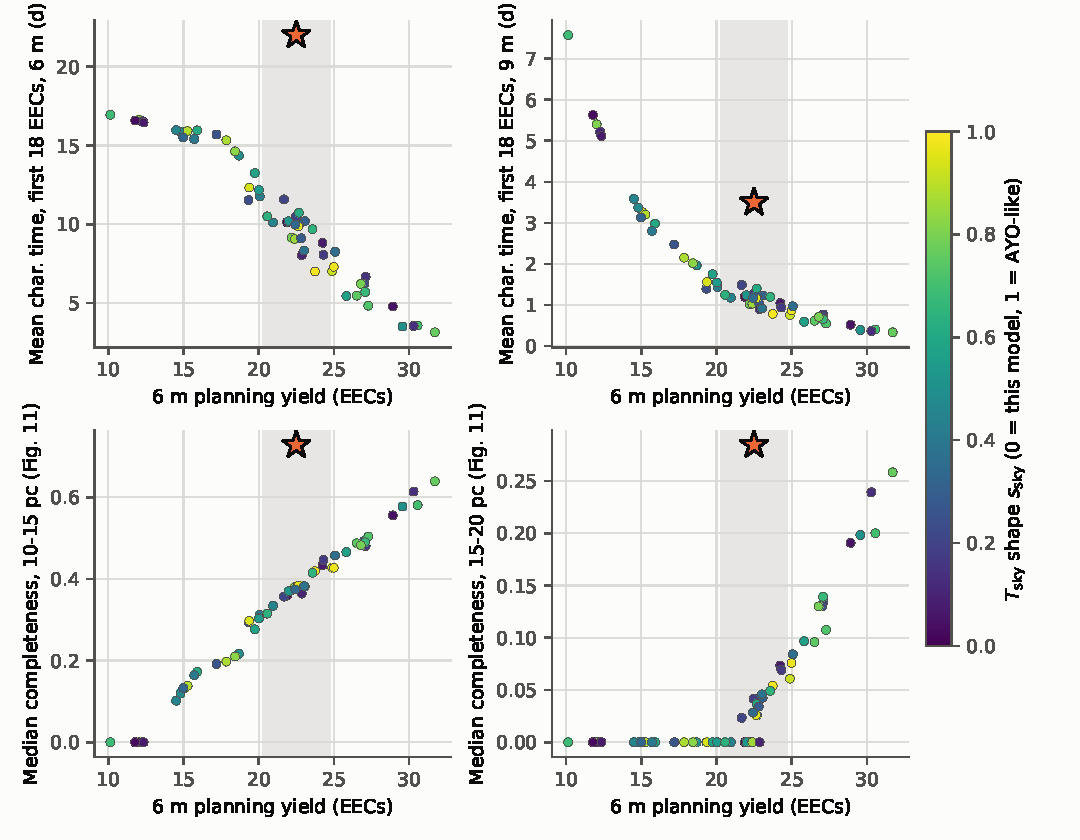
\includegraphics[width=\textwidth]{figCalibrationDegeneracyObservables.pdf}
\caption{Every one of the 56 settings of the throughput study, plotted as a published
observable against the $6\,$m planning yield and colored by the $T_{\rm sky}$ shape parameter
$s_{\rm sky}$. The star marks Stark et al.\ (2024)'s published pair of values; the shaded band is
the published yield $\pm10\%$. A setting that reproduced Stark would place a point on the star in
all four panels. Instead, the points in each panel lie on one narrow curve set by the yield, with
the $T_{\rm sky}$ shape mixed along it, and the characterization times at both apertures and the
completeness at 10--15\,pc miss the published values at the published yield.}
\label{fig:degobs}
\end{figure}

\begin{figure}[htbp]
\centering
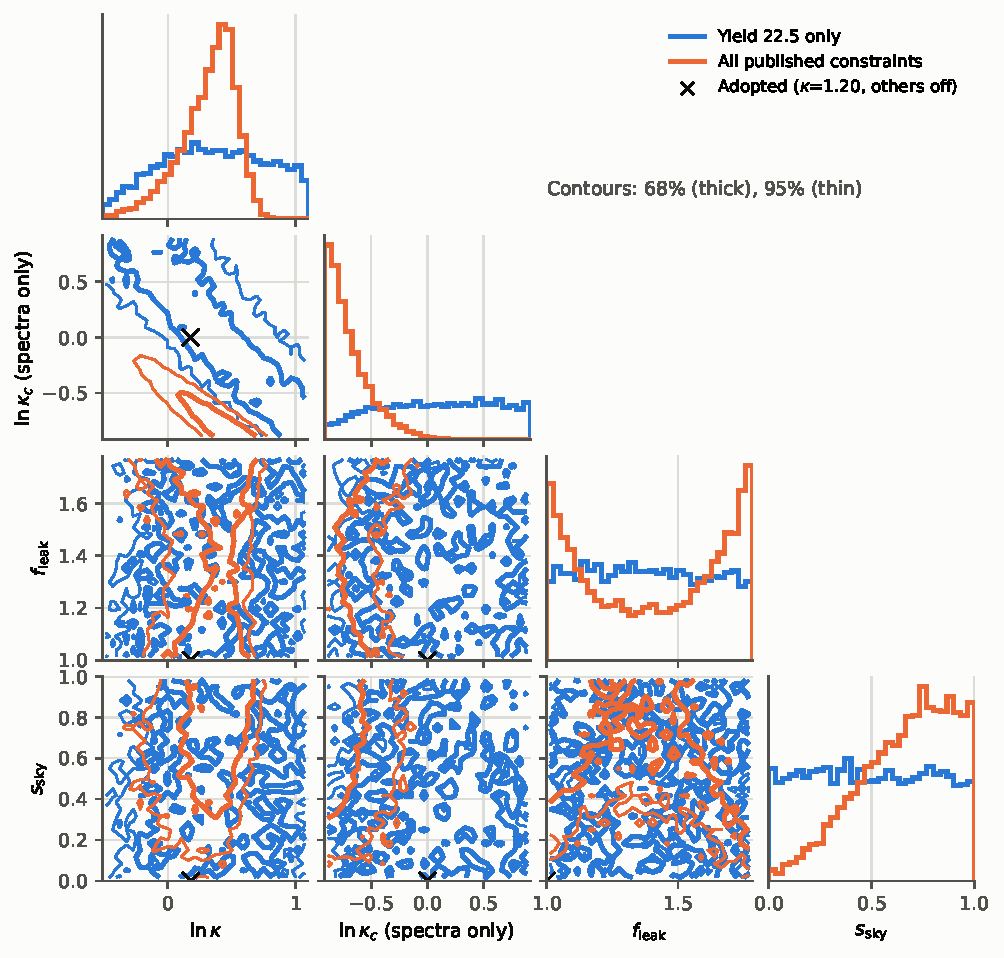
\includegraphics[width=0.85\textwidth]{figCalibrationDegeneracyCorner.pdf}
\caption{Posteriors over the four throughput-family parameters, from a quadratic emulator of the
56-point design whose leave-one-out error is folded into the tolerance so that emulator
error cannot pose as a constraint. Blue: constrained on the published $6\,$m yield alone. Orange:
constrained on the yield, the characterization times at 6 and $9\,$m, and the Fig.~11 completeness
in three distance bins. The $\ln\kappa$--$\ln\kappa_c$ panel shows the degeneracy that the
published observables leave open; the orange contours run into the prior boundary on $\kappa_c$
while still failing to reach the published characterization times.}
\label{fig:corner}
\end{figure}

\subsection{What this implies}

We can state the disagreement sharply, which is what makes it a question rather than a complaint.
Our exposure-time equations reproduce AYO's. Our count rates reproduce AYO's. AYO's own published
ETC gives Earth-twin spectra at 12--18~pc that take 37--104~d. The two-month cap is stated. And
yet Stark et al. (2024) Fig.~11 shows those stars reaching habitable-zone completeness of
0.5--0.8. We cannot construct a survey in which both are true. Within the four throughput
parameters that could plausibly absorb the difference, over the ranges above, no setting makes
them both true: Fig.~\ref{fig:degobs} shows every setting we ran, and none lands on the published
values.

The resolution is therefore something about how AYO counts or charges characterization within the
survey that is not in the papers we have. That is Question~1 (Sec.~\ref{sec:discussion}).

%======================================================================
\section{Second discrepancy: the reading of the occurrence interval}
\label{sec:eta}
%======================================================================

\subsection{One sentence, two readings}

Stark et al. (2024) Sec.~3.6 states:
\begin{quote}
\emph{``Performing this computation for each element of our posterior, we get an $\eta_\oplus$
with mean and 86\% confidence interval $\eta_\oplus = 0.26^{+0.29}_{-0.14}$.''}
\end{quote}
The underlying distribution is built by uniformly mixing the two completeness-extrapolation cases
of Bryson et al. (2021), and is described as having a tail of large $\eta_\oplus$ values.

Propagating this requires two interpretive decisions that the sentence does not settle for a
reader building a parametric law. Is $0.26$ the mean, as stated, or the center of the quoted
interval? And is $[0.12, 0.55]$ an 86\% interval, as stated, or the 68\% that is the near-universal
convention and a digit transposition away?

\textbf{What we adopt.} We read $[0.12, 0.55]$ as a \emph{68\%} (one-sigma) interval, not the
stated 86\%, and we treat its center as the \emph{median}, not the stated mean. Concretely,
$\eta_\oplus$ is lognormal (Eq.~\ref{eq:etalaw}) with $z = 1$: its median is
$\sqrt{0.12 \times 0.55} = 0.257$, the geometric center of the interval, its $\ln$-width is
0.76, and its mean is 0.343, above the stated 0.26. Both choices depart from the
text.

We flag this prominently because it is the kind of choice that reproductions usually bury. It was
adopted because it reproduces the published Fig.~10, and a choice adopted because it reproduces
the target is exactly the kind of choice that has to be justified on other grounds or declared.

\subsection{A factorial decomposition}

Our pipeline follows Stark's documented albedo method, and departs from a fully text-faithful
reading in one setting: the interval reading above. To test whether that departure stands alone,
we pair it with the albedo method, which is the other setting a reproduction could plausibly
choose differently: re-deriving each drawn-albedo planet's exposure time instead of Stark's
per-visit flux test. The two settings form a complete $2\times2$, which we evaluated end to end
(Table~\ref{tab:variants}).

The decomposition is unambiguous. On the total-variation distance $D_{\rm TV}$ to the published
Fig.~10, the
interval reading is worth +0.0936, the albedo method -0.0009, and the interaction
+0.0006. \textbf{The interval reading accounts for 99.1\% of the disagreement and
the albedo method 0.9\%.} The albedo method affects the agreement with Fig.~10 hardly
at all; it matters only for the albedo penalty (3.6\% with Stark's test,
8.6\% with re-derived exposures, against a published 12\%).

\begin{table}[htbp]
\centering
\small
\begin{tabular}{lccccc}
\toprule
\textbf{Model} & \textbf{Peak} & \textbf{Mean} & \textbf{$P(Y<12)$} & \textbf{$D_{\rm TV}$ to Fig.~10} &
\textbf{Yield ratio} \\
\midrule
Adopted                              & 12  & 22.4  & 0.26  & 0.037  & 0.2315 \\
$\eta_\oplus$ as 86\% (every documented choice) & 15 & 20.6 & 0.19 & 0.131 & 0.2292 \\
Albedo: exposure re-derived          & 11   & 21.0   & 0.28   & 0.038   & 0.2386 \\
Albedo re-derived and 86\%           & 15  & 19.5  & 0.22  & 0.132  & 0.2363 \\
Constant $T_{\rm sky}$               & 10   & 19.2   & 0.34   & 0.089   & 0.2225 \\
86\% and constant $T_{\rm sky}$      & 12  & 17.4  & 0.30  & 0.146  & 0.2201 \\
Stark's own $\eta_\oplus$ law        & 7   & 17.8   & 0.41   & 0.155   & 0.2279 \\
\midrule
Stark et al. (2024)                    & 10   & 21.0             & 0.29              & ---            & --- \\
\bottomrule
\end{tabular}
\caption{Seven models, each differing from the adopted one in named settings, evaluated end to
end with every other setting, input file and random seed held fixed and nothing fitted.
``Peak'' is the mode of the exact Poisson mixture (Eq.~\ref{eq:mixture}), and $D_{\rm TV}$ the
total-variation distance to Stark's purple curve (Eq.~\ref{eq:dtv}; smaller is better). The last
column is the deliverable of
Sec.~\ref{sec:result}; it stays between 0.2201 and 0.2386 across the whole
table.}
\label{tab:variants}
\end{table}

\subsection{Following every documented choice makes the agreement worse}

The natural response to a reproduction that departs from its source in two places is to demand
that it stop departing. We did that, and it fails (Fig.~\ref{fig:peaks}). With the albedo test
already Stark's, adopting the stated 86\% interval as well gives a model that follows every
documented choice. It moves the peak from 12 to 15 against a published
10, and the total-variation distance from 0.037 to 0.131.

This is the central empirical fact of this section, and we do not think it is a comfortable one
for either side. Read one way it says our model is wrong in a manner that only the 68\% reading
happens to compensate. Read the other way it says the published text and the published figure are
not mutually consistent, and that the figure is the better guide to what was computed. We present
evidence below for the second reading, but we want to be explicit that the first cannot be
excluded by anything we have.

\begin{figure}[htbp]
\centering
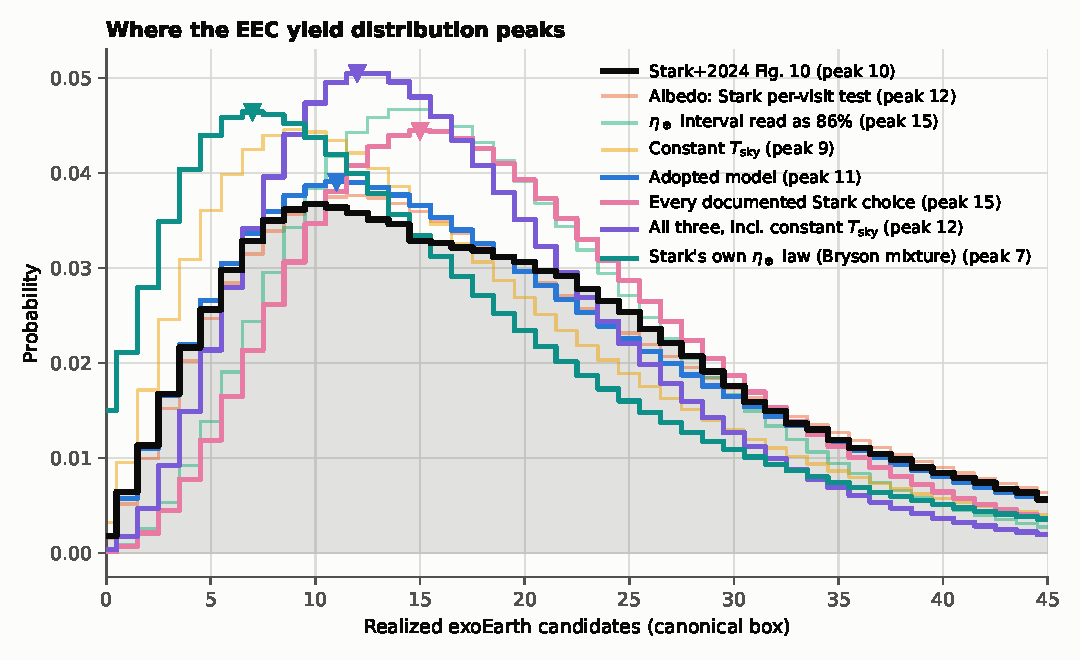
\includegraphics[width=0.95\textwidth]{figYieldPeakComparison.pdf}
\caption{Realized EEC yield distributions for every model of Table~\ref{tab:variants}, against
the digitized Stark et al. (2024) Fig.~10 (heavy black). Each curve is the exact Poisson mixture
over that model's sampled expected yields. The one-at-a-time probes are drawn back; the combined
models carry peak markers.}
\label{fig:peaks}
\end{figure}

\subsection{Testing the interval against its own source}

The reading can be tested without reference to our yield model at all, by asking what the quoted
interval means for the distribution it is quoted from. We took the two Bryson et al. (2021) cases,
mixed them uniformly as Stark et al. (2024) describes, and rescaled the mixture by the single factor
that sets its mean to the stated 0.26. No parameter is fitted.

That distribution puts 59\% of its mass inside the quoted $[0.12, 0.55]$. Its own 68\%
interval is $[0.076, 0.429]$ and its own 86\% interval is
$[0.047, 0.653]$ --- the latter far wider than what is printed. Its median is
0.183 when its mean is 0.26, which is strongly right-skewed and therefore inconsistent
with reading $0.26$ as a median, as our pipeline does.

Two conclusions follow. The quoted interval is much closer to a 68\% interval of its own source
than to an 86\% one, which supports the transposition reading. But the mixture is also not a
lognormal, and its shape cannot be represented by one: no lognormal can simultaneously carry the
stated mean, the stated interval and any single confidence level. Our 68\% reading may therefore
not be a corrected typo at all --- it may be a width that compensates for a tail our functional
form does not have. Those two explanations are observationally identical in the figure agreement,
which is precisely why the agreement alone never justified the choice.

We tested the obvious remedy: replacing the lognormal with Stark's own construction, the rescaled
Bryson mixture, as the occurrence law. It does not work either. That model peaks at 7
against a published 10 and has the largest total-variation distance of any model we have
built (0.155). We believe this reflects our shape transfer rather than his method:
Bryson's published distribution is for his own radius and effective-temperature selection, while
Stark recomputed $\eta_\oplus$ from Bryson's chains over a different one, and rescaling transfers
the first moment but not the shape. The three candidate laws bracket the published curve --- the
Bryson mixture at 7, the 68\% lognormal at 12, the 86\% lognormal at
15, against 10 --- and we cannot choose among them from published information.

That is Question~2 (Sec.~\ref{sec:discussion}).

%======================================================================
\section{The counterfactual, and its robustness}
\label{sec:result}
%======================================================================

We now answer the question that motivated the reimplementation: what the baseline HWO mission
would find if exoEarth candidates were defined by mass, $0.5$--$2\,M_\oplus$ with $R = M^{0.27}$,
in a habitable zone of $0.96$--$1.20$~AU scaled as $\sqrt{L_\star}$.

The occurrence rate over the redefined box is 0.0520 against 0.255 over the canonical
one, a ratio of 0.204. The median realized canonical yield is 18.8 (90\% interval
5.6--53.4) and the median redefined yield is 4.3
(1.2--14.8). The yield ratio, with its 68\% interval, is
\[
  \frac{Y_{\rm redefined}}{Y_{\rm canonical}} = 0.232^{+0.027}_{-0.021}.
\]
The probability of reaching 25 candidates falls from 35.1\% to 1.20\%.

\begin{figure}[htbp]
\centering
\begin{minipage}{0.48\textwidth}\centering\textbf{This work}\\[2pt]
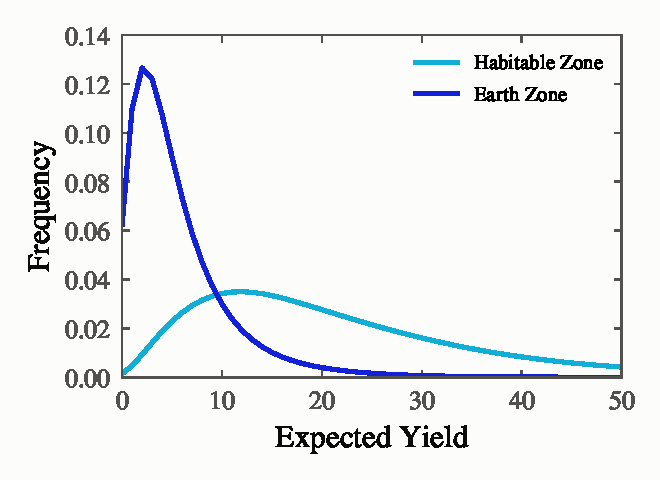
\includegraphics[width=\linewidth]{figYieldZoneDistributions.pdf}\end{minipage}\hfill
\begin{minipage}{0.48\textwidth}\centering\textbf{Stark et al.\ (2024) Fig.~10}\\[2pt]
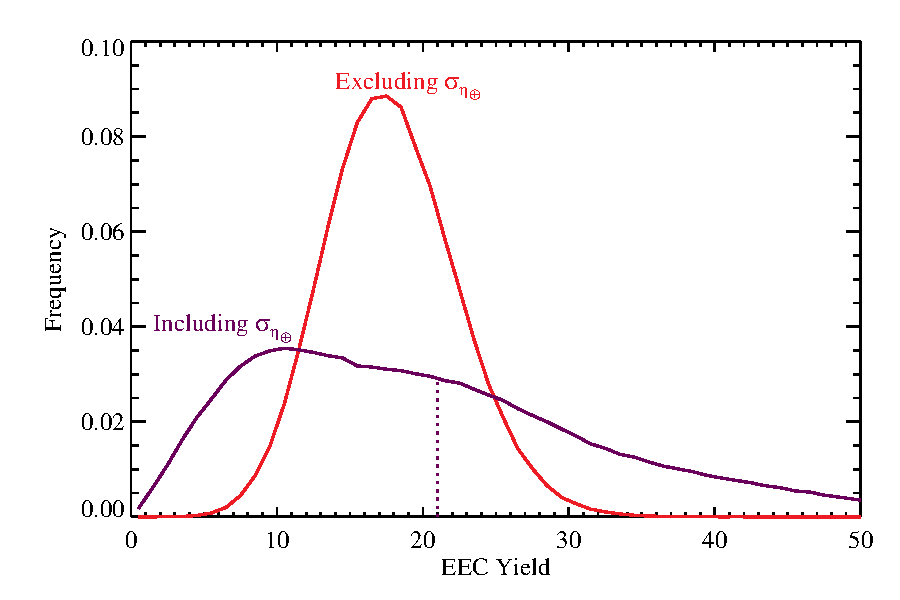
\includegraphics[width=\linewidth]{../ComparePublishedFigures/reference/starkFigure10.pdf}\end{minipage}
\caption{Left: EEC yield distributions for the canonical habitable-zone selection (pale blue) and
for the narrowed, mass-selected Earth zone (dark blue), marginalized over the occurrence posterior
and the exozodi draws and including exoplanet sampling uncertainty. Each curve is the exact Poisson
mixture over the sampled expected yields. Right: the published distributions for the canonical
selection, copied unaltered from the arXiv source. Our pale blue curve is the counterpart of
Stark's purple curve (``Including $\sigma_{\eta_\oplus}$''), not his red one: both describe the
same selection, the same $6\,$m design and the same sources of uncertainty (the spread in
$\eta_\oplus$, exozodi, albedo and planet sampling). They should share a broad peak near 10, a mean
near 21 and a long tail toward high yields; ours peaks at 12 (published 10),
with mean 22.4 (21.0), median 19 (18), $P(Y<12) = 0.26$ (0.29),
and a total-variation distance of 0.037 between the two curves. Stark's red curve holds
$\eta_\oplus$ fixed (``Excluding $\sigma_{\eta_\oplus}$''), which removes most of the spread; its
counterpart in this model is the fixed-$\eta_\oplus$ distribution, with mean 17.73 against
his 17.35, and it is not drawn here. The Earth zone has no published counterpart. The
yield range follows Stark's Fig.~10; our abscissa is labeled in plain English rather than with
his ``EEC yield''.}
\label{fig:zones}
\end{figure}

The yield ratio exceeds the occurrence ratio, which is at first sight surprising and is real. Two
effects contribute: fewer expected detections free characterization time, which the optimizer
reallocates; and truncating the outer habitable zone preferentially removes the faintest, most
expensive planets, so the candidates that survive are cheaper per detection.

\textbf{The result is robust to both open questions.} This is the reason we are willing to report
it while Secs.~\ref{sec:char} and~\ref{sec:eta} remain open. Across the seven models of
Table~\ref{tab:variants} --- which span both readings of the occurrence interval, both albedo
methods, the presence and absence of the $T_{\rm sky}$ term, and a completely different functional
family for the occurrence law --- the yield ratio spans 0.2201 to 0.2386, inside
the 68\% interval of the adopted value. The ratio
is a comparison between two selections evaluated in the same model, and the systematics that
trouble the absolute yield largely divide out of it.

%======================================================================
\section{Discussion: the two questions}
\label{sec:discussion}
%======================================================================

We have described a reproduction that succeeds on most of the published record and fails on two
points. We now argue that those two points are not a list of remaining work but the hinge of the
whole exercise, and that each reduces to a question of fact that one email can settle.

\subsection*{Question 1. How does the AYO baseline survey characterize its 10--20~pc targets
within the two-month limit?}

Stark et al. (2024) Fig.~11 shows habitable-zone completeness of 0.5--0.8 for targets at 10--20~pc.
AYO's own exposure-time calculator (Stark et al. 2025) gives Earth-twin spectra at those distances
of 37--104~d. The characterization limit is two months. We reproduce the ETC to 0.94--1.02 on
AYO's own inputs, and across the four throughput parameters that could absorb the difference,
including a $T_{\rm sky}$ shaped like AYO's, no setting we ran does (Sec.~\ref{sec:char},
Fig.~\ref{fig:degobs}). Either those stars are characterized under conditions more favorable than
an Earth twin at maximum elongation, or the completeness plotted in Fig.~11 is not gated on
characterization, or characterization is charged to the budget differently from the way we charge
it, or AYO's DMVC6 $T_{\rm sky}$ map departs from ours by more than its vortex benchmark suggests
(Sec.~\ref{sec:tsky}). Any of these would be a one-sentence answer, and each implies a different
correction.

\subsection*{Question 2. In Sec.~3.6, is $\eta_\oplus = 0.26$ the mean or the median, and is
$[0.12, 0.55]$ an 86\% or a 68\% interval?}

The text says mean and 86\%. Our pipeline uses median and 68\%, and that combination reproduces
the published Fig.~10 while the stated combination does not (Sec.~\ref{sec:eta}). The quoted
interval contains 59\% of the mass of its own source distribution, which is much
nearer 68\% than 86\%. ``86'' is a digit transposition of ``68'', and the phrase occurs exactly
once in the paper, which otherwise quotes standard deviations throughout. We are not in a position
to assert a typographical error in someone else's paper on that evidence, and we do not. But the
question is answerable immediately by the authors, and nothing else we can do resolves it.

\subsection*{Why the reproduction hinges on these}

It would be possible to read the preceding sections as a report of two modest residuals in an
otherwise successful reproduction. We think that reading is wrong, for three reasons.

\emph{First, they control the quantities that matter for mission design.} The characterization
time budget determines the target mix, and the target mix determines which stars must be
surveyed for exozodi in advance, which drives a precursor-mission argument. The occurrence
interval controls the width of the yield distribution, and the width determines
$P(Y \ge 25)$, which is the quantity the decadal recommendation is written in. A reproduction
that matches the mean yield but not the width does not reproduce the statement the mission is
designed against.

\emph{Second, the agreement we do have is partly contingent on the choices in question.} Our
agreement with the shape of Fig.~10 holds under the 68\% reading and fails under the 86\%
one. We cannot simultaneously claim that our model is validated by that
agreement and that the reading which produces it is an open question. Honesty requires reporting
the agreement as conditional, and Question~2 is the condition.

\emph{Third, the two are not independent in their consequences.} Both act on the same downstream
quantity. The characterization-time discrepancy moves the target mix and hence the level; the
occurrence reading moves the width. A reader trying to judge whether our model is fit for a given
purpose needs both answered, because a model with the right level and the wrong width and a model
with the wrong level and the right width fail different applications.

We therefore present this work not as a completed reproduction with caveats, but as a
reproduction that has been carried as far as the published record permits, together with the two
specific facts that would carry it the rest of the way.

\subsection*{What we are not claiming}

We are not claiming an error in AYO. Every discrepancy reported here is equally consistent with an
error in our reimplementation that we have failed to find, and we have found and fixed seventeen
such errors already (Appendix~\ref{app:ledger}); there is no reason to believe the count is
final. What we do claim is narrower and, we think, defensible: that the published description is
not sufficient to determine these two quantities, and that we have exhausted the interpretations
available to us.

%======================================================================
\section{Conclusions}
%======================================================================

\begin{enumerate}
\item An independent reimplementation of AYO, built from the published equations and parameters
  with no parameter fitted to the published yield, reproduces the Stark et al. (2024) baseline
  $6\,$m exoEarth candidate yield to 7.0\% and agrees with 21 of
  24 independent published comparisons.
\item The realized-yield distribution reproduces the shape of the published one (total-variation
  distance 0.037). The peak should be computed as an exact Poisson mixture; the mode of a
  histogram of realized draws is too noisy to support the comparison.
\item Stark's own per-visit albedo test, adopted here, gives an albedo penalty of 3.6\%
  against the 12\% he reports.
\item Spectral characterization times remain too steep in target difficulty and aperture. A
  56-point factorial design establishes that no member of the throughput-parameter
  family reaches the published characterization times at the published yield.
\item The $\eta_\oplus$ interval of Sec.~3.6 admits two readings that differ materially. A
  $2\times2$ decomposition attributes 99.1\% of the residual disagreement with the
  published yield distribution to that single choice, and following every documented choice
  simultaneously makes the agreement worse rather than better.
\item Both residues reduce to questions of fact that the AYO authors can answer in a sentence, and
  we state them explicitly in Sec.~\ref{sec:discussion}.
\item For the counterfactual that motivated the work --- a mass-selected sample in a narrowed
  habitable zone --- the yield ratio is $0.232^{+0.027}_{-0.021}$ (68\%
  interval), and it stays between 0.2201 and 0.2386 across every model variant
  spanning both open questions.
\end{enumerate}

%======================================================================
\appendix
\section{Verification against the published record}
\label{app:verification}
%======================================================================

\begin{table}[htbp]
\centering
\scriptsize
\begin{tabular}{p{5.4cm}rrrrl}
\toprule
\textbf{Check} & \textbf{Published} & \textbf{Model} & \textbf{Diff.} & \textbf{Tol.} & \textbf{Verdict} \\
\midrule
eta\_Earth over the canonical box (SAG13) & 0.24 & 0.2404 & 0\% & 3\% & agrees \\
Uncalibrated 6 m yield & 22.5 & 20.92 & 7\% & 20\% & agrees \\
Throughput factor needed to reach 22.5 & 1 & 1.195 & 20\% & 100\% & agrees \\
Sampling distribution mean (Fig. 4) & 22.5 & 20.91 & 7\% & 20\% & agrees \\
Sampling distribution sigma (Fig. 4) & 5 & 4.567 & 9\% & 25\% & agrees \\
Albedo penalty on expected yield & 0.12 & 0.03608 & 70\% & 50\% & \textbf{disagrees} \\
P25 including sigma\_eta, 6 m & 0.32 & 0.3514 & 10\% & 25\% & agrees \\
Yield-aperture exponent & 1.9 & 1.813 & 5\% & 15\% & agrees \\
Exozodi-sampling penalty on expected yield & 0.111 & 0.1217 & 10\% & 50\% & agrees \\
P25 excluding sigma\_eta, 6 m & 0.06 & 0.06264 & 4\% & 50\% & agrees \\
Mean characterization time, first 18 EECs, 6 m (days) & 22 & 14.34 & 35\% & 30\% & \textbf{disagrees} \\
Mean characterization time, first 18 EECs, 9 m (days) & 3.5 & 2.053 & 41\% & 30\% & \textbf{disagrees} \\
Characterization-time ratio 6 m / 9 m & 6.2 & 6.987 & 13\% & 20\% & agrees \\
P25 including sigma\_eta at 6 m & 0.32 & 0.3508 & 10\% & 25\% & agrees \\
P25 including sigma\_eta at 7 m & 0.53 & 0.5271 & 1\% & 25\% & agrees \\
P25 including sigma\_eta at 8 m & 0.67 & 0.6573 & 2\% & 25\% & agrees \\
P25 including sigma\_eta at 9 m & 0.78 & 0.755 & 3\% & 25\% & agrees \\
Fixed-eta yield mean (Fig. 10 red) & 17.35 & 17.73 & 2\% & 10\% & agrees \\
Realized-yield distribution median & 18 & 19 & 6\% & 15\% & agrees \\
Realized-yield fraction below 12 EECs & 0.2907 & 0.2597 & 11\% & 35\% & agrees \\
Realized-yield distribution mean & 21 & 22.45 & 7\% & 30\% & agrees \\
Realized-yield distribution mode & 10 & 11 & 10\% & 25\% & agrees \\
Maximum luminosity among reachable targets & 20 & 12.5 & 38\% & 60\% & agrees \\
Maximum distance among reachable targets & 25 & 22.02 & 12\% & 60\% & agrees \\
\bottomrule
\end{tabular}
\caption{The 24 independent comparisons of step A09, of which 21 agree. Published
values taken from Fig.~10 are digitized from the figure's vector content stream. Comparisons
against quantities that entered the model as inputs are tagged as tuned and excluded from the
count.}
\label{tab:verif}
\end{table}

%======================================================================
\section{Published figures beside their model counterparts}
\label{app:pairs}
%======================================================================

\begin{figure}[htbp]
\centering
\begin{minipage}{0.48\textwidth}\centering\textbf{Stark et al.\ (2024) Fig.~4}\\[2pt]
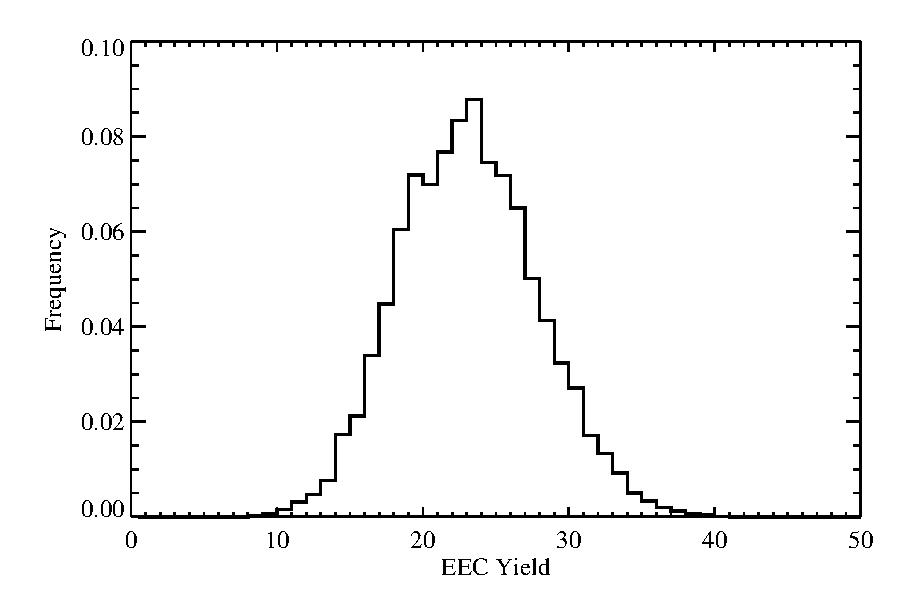
\includegraphics[width=\linewidth]{../ComparePublishedFigures/reference/starkFigure04.pdf}\end{minipage}\hfill
\begin{minipage}{0.48\textwidth}\centering\textbf{This model}\\[2pt]
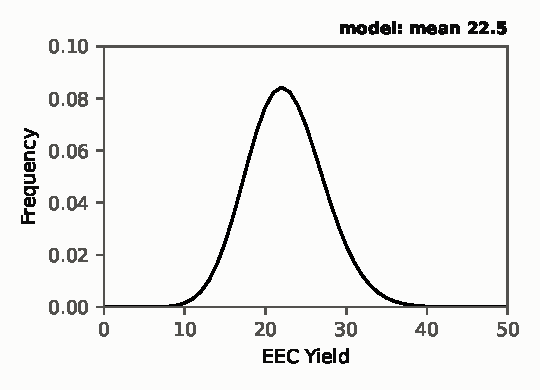
\includegraphics[width=\linewidth]{figMatchStarkFig04.pdf}\end{minipage}
\caption{Planet sampling as the only source of uncertainty: $A_G = 0.2$, exozodi fixed at 3 zodis, and Poisson counting of planets. Published: mean 22.5, standard deviation 21\% of the mean. Model: mean 20.9, with nothing fitted to the published yield.}
\label{fig:pair04}
\end{figure}

\begin{figure}[htbp]
\centering
\begin{minipage}{0.48\textwidth}\centering\textbf{Stark et al.\ (2024) Fig.~7}\\[2pt]
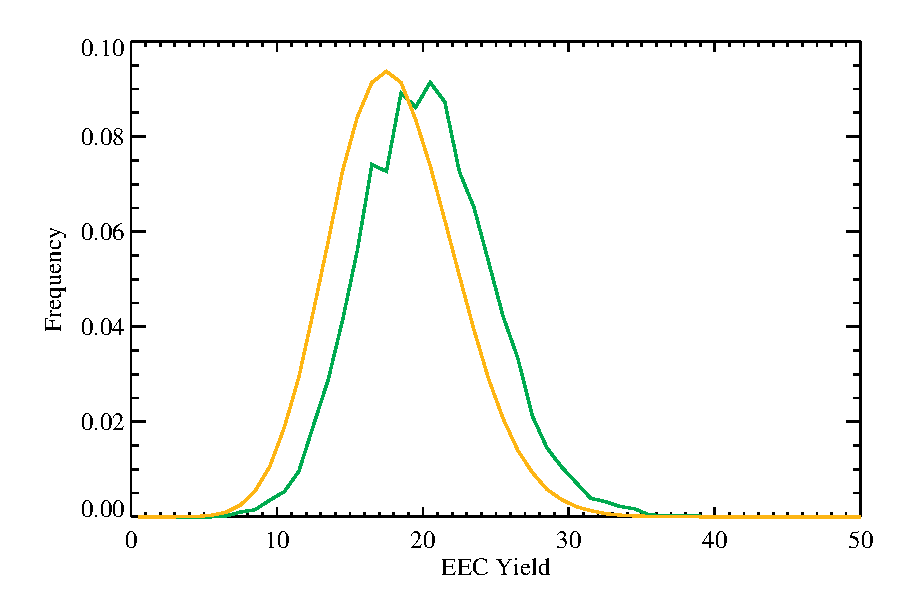
\includegraphics[width=\linewidth]{../ComparePublishedFigures/reference/starkFigure07.pdf}\end{minipage}\hfill
\begin{minipage}{0.48\textwidth}\centering\textbf{This model}\\[2pt]
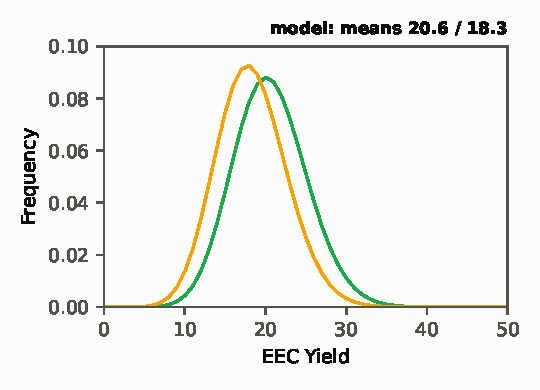
\includegraphics[width=\linewidth]{figMatchStarkFig07.pdf}\end{minipage}
\caption{Yield with albedo drawn and exozodi fixed (green), and with exozodi drawn as well (orange), both at fixed $\eta_\oplus$. Published means: 19.8 and 17.6. Model means: 20.1 and 17.7, over 200 draws.}
\label{fig:pair07}
\end{figure}

\begin{figure}[htbp]
\centering
\begin{minipage}{0.48\textwidth}\centering\textbf{Stark et al.\ (2024) Fig.~9}\\[2pt]
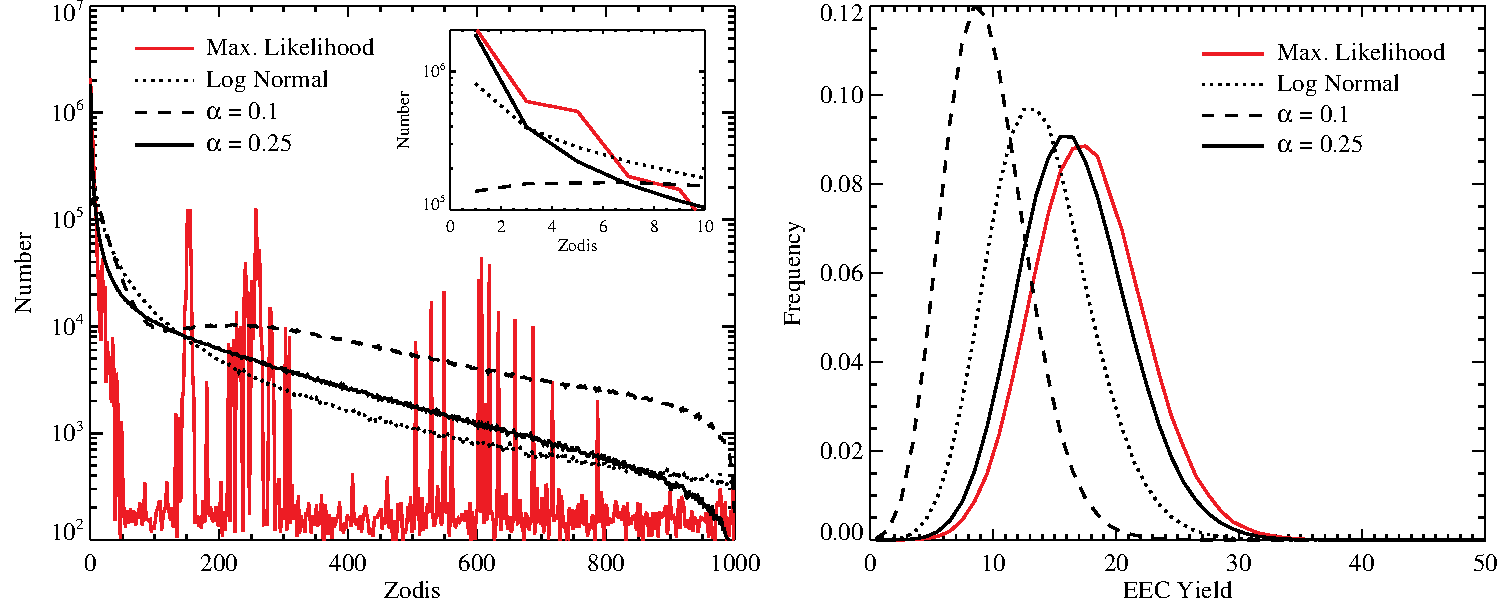
\includegraphics[width=\linewidth]{../ComparePublishedFigures/reference/starkFigure09.pdf}\end{minipage}\hfill
\begin{minipage}{0.48\textwidth}\centering\textbf{This model}\\[2pt]
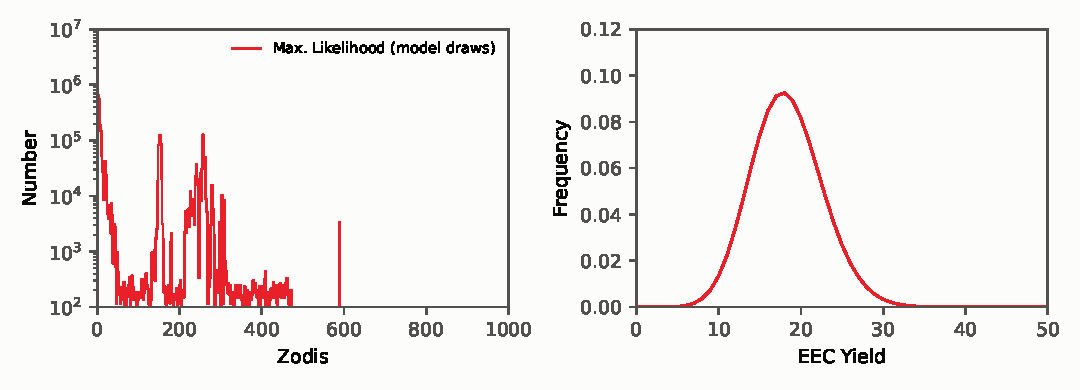
\includegraphics[width=\linewidth]{figMatchStarkFig09.pdf}\end{minipage}
\caption{Left: exozodi levels drawn from the LBTI HOSTS maximum-likelihood distribution (red). The model panel is a histogram of the levels the pipeline actually drew, scaled to Stark's $500\times10^4$ draws; its median is 3.00 zodis. Stark's other three distributions are not modeled. Right: the yield those levels produce at fixed $\eta_\oplus$ (red).}
\label{fig:pair09}
\end{figure}

\begin{figure}[htbp]
\centering
\begin{minipage}{0.48\textwidth}\centering\textbf{Stark et al.\ (2024) Fig.~10}\\[2pt]
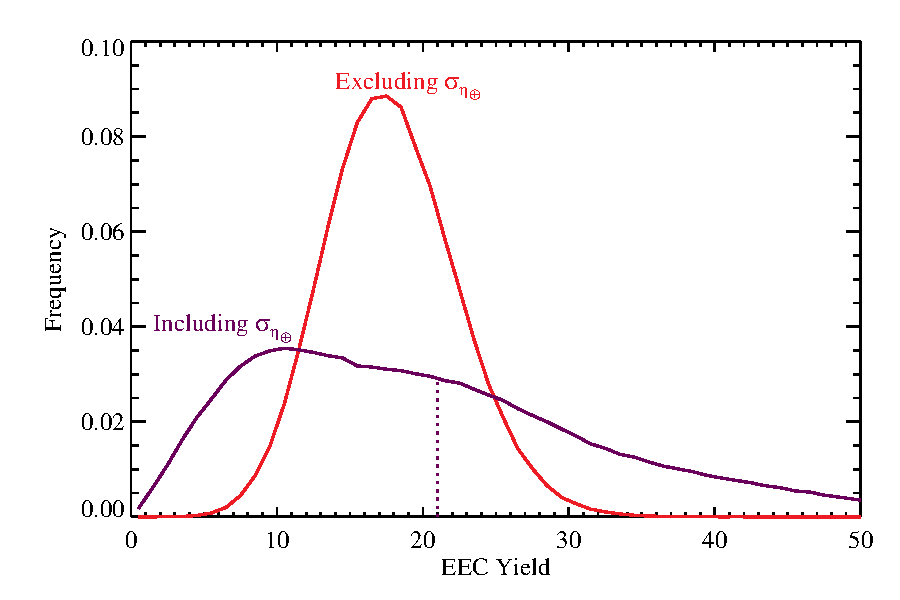
\includegraphics[width=\linewidth]{../ComparePublishedFigures/reference/starkFigure10.pdf}\end{minipage}\hfill
\begin{minipage}{0.48\textwidth}\centering\textbf{This model}\\[2pt]
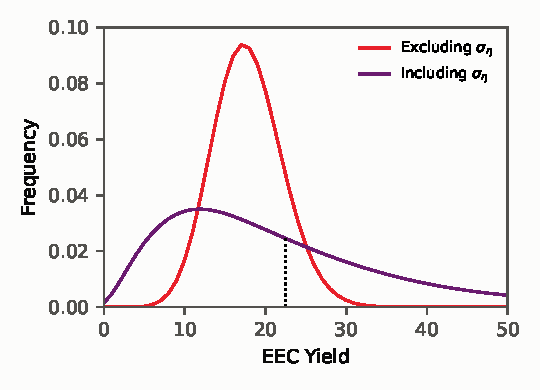
\includegraphics[width=\linewidth]{figMatchStarkFig10.pdf}\end{minipage}
\caption{Realized yield including (purple) and excluding (red) the uncertainty in $\eta_\oplus$; the dotted line marks the mean of the purple curve. Total-variation distance between model and published curves: 0.027 (purple) and 0.052 (red). Means (purple / red): published 21.0 / 17.3, model 22.5 / 17.8.}
\label{fig:pair10}
\end{figure}

\begin{figure}[htbp]
\centering
\begin{minipage}{0.48\textwidth}\centering\textbf{Stark et al.\ (2024) Fig.~11}\\[2pt]
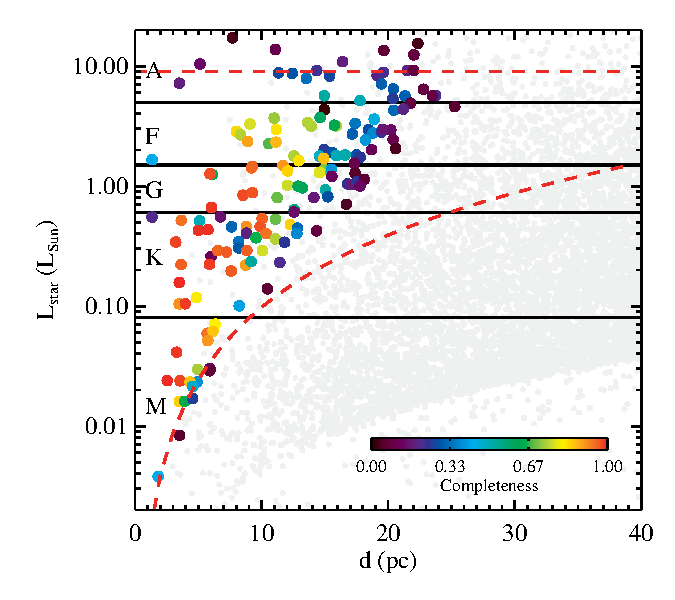
\includegraphics[width=\linewidth]{../ComparePublishedFigures/reference/starkFigure11.pdf}\end{minipage}\hfill
\begin{minipage}{0.48\textwidth}\centering\textbf{This model}\\[2pt]
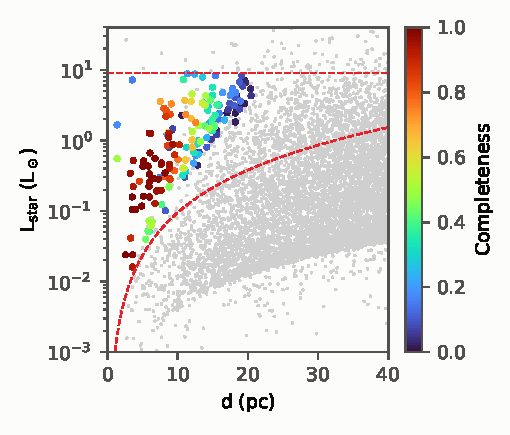
\includegraphics[width=\linewidth]{figMatchStarkFig11.pdf}\end{minipage}
\caption{Targets selected in one representative exozodi draw, colored by completeness and plotted over the full input list (gray). Both panels use Stark's own color scale, read from the color bar embedded in the published figure. Published: 154 targets, summed completeness 77.4, median 0.50. Model (draw 14, the draw with the median yield): 157 targets, summed completeness 77.0, and median 0.09 over the 141 targets that match. The red dashed lines are the noise floor for a 1.4\,$R_\oplus$ planet at the EEID, and the outer edge of the habitable zone at 1.5\,$\lambda/D$ at 1\,$\mu$m. The spectral-type lines are not redrawn.}
\label{fig:pair11}
\end{figure}

\begin{figure}[htbp]
\centering
\begin{minipage}{0.48\textwidth}\centering\textbf{Stark et al.\ (2024) Fig.~12}\\[2pt]
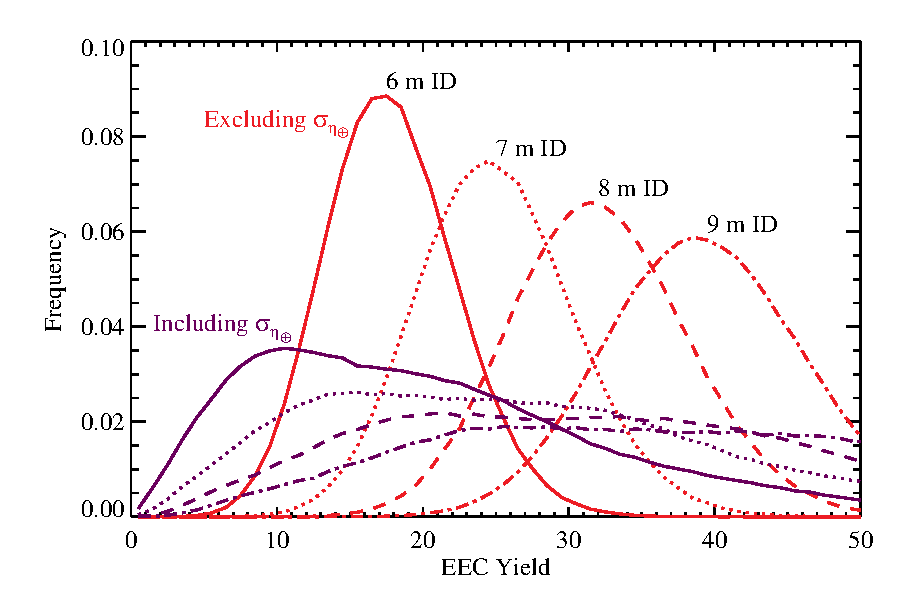
\includegraphics[width=\linewidth]{../ComparePublishedFigures/reference/starkFigure12.pdf}\end{minipage}\hfill
\begin{minipage}{0.48\textwidth}\centering\textbf{This model}\\[2pt]
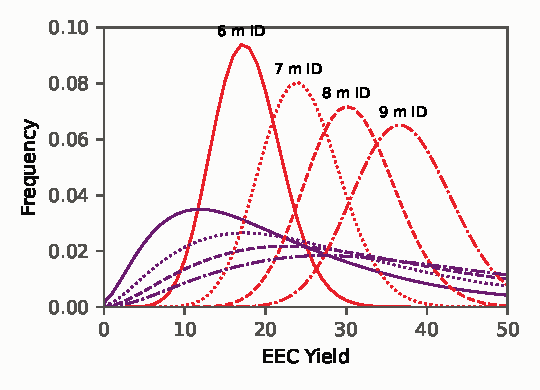
\includegraphics[width=\linewidth]{figMatchStarkFig12.pdf}\end{minipage}
\caption{Realized yield at inscribed diameters of 6, 7, 8 and 9\,m (solid, dotted, dashed and dot-dashed), including (purple) and excluding (red) the uncertainty in $\eta_\oplus$, with no calibration at any aperture. Excluding that uncertainty, Stark's 9\,m yield is 2.2 times his 6\,m yield; the model's is 2.09 times.}
\label{fig:pair12}
\end{figure}

\begin{figure}[htbp]
\centering
\begin{minipage}{0.48\textwidth}\centering\textbf{Stark et al.\ (2024) Fig.~14}\\[2pt]
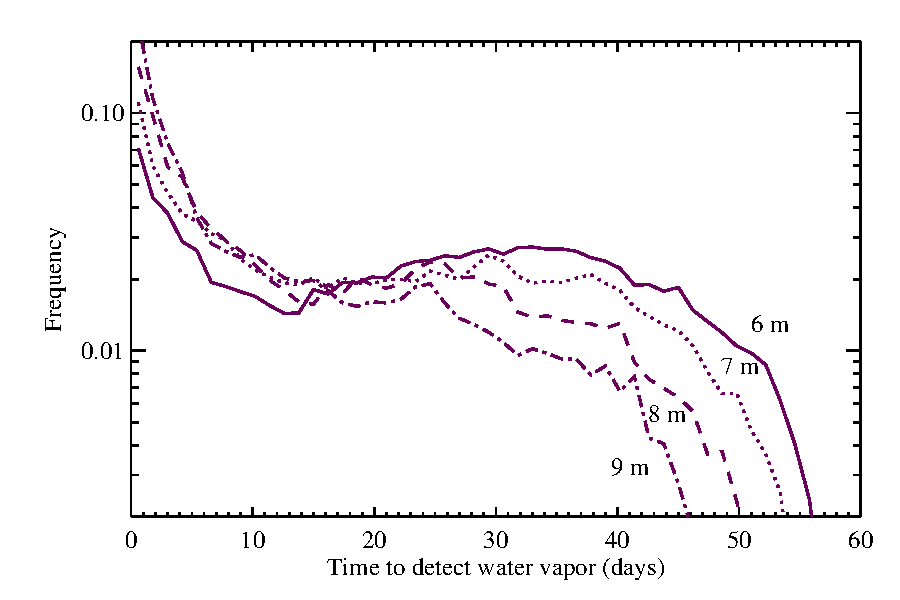
\includegraphics[width=\linewidth]{../ComparePublishedFigures/reference/starkFigure14.pdf}\end{minipage}\hfill
\begin{minipage}{0.48\textwidth}\centering\textbf{This model}\\[2pt]
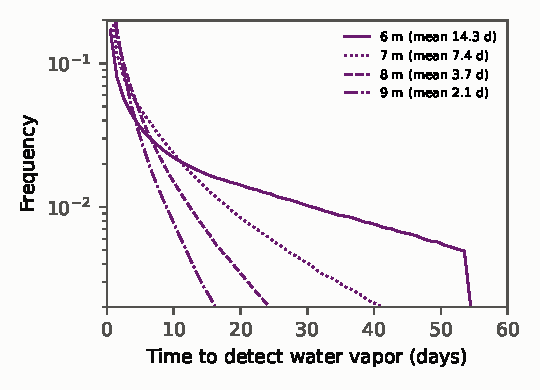
\includegraphics[width=\linewidth]{figMatchStarkFig14.pdf}\end{minipage}
\caption{Characterization times of the individual EECs among the first 18, at 6--9\,m. The model uses 20 exozodi draws, recomputed planet by planet, in 1-day bins. Published means: 22 days at 6\,m and 3.5 days at 9\,m. Model means at 6/7/8/9\,m: 14.3 / 7.4 / 3.7 / 2.1 days. Stark does not state how his histograms are normalized, and with 1-day bins his 9\,m plateau alone would exceed his stated mean, so compare the shapes rather than the heights. His distributions keep a plateau of 15--50-day spectra at every aperture; the model's do not.}
\label{fig:pair14}
\end{figure}

\begin{figure}[htbp]
\centering
\begin{minipage}{0.48\textwidth}\centering\textbf{Stark et al.\ (2024) Fig.~15}\\[2pt]
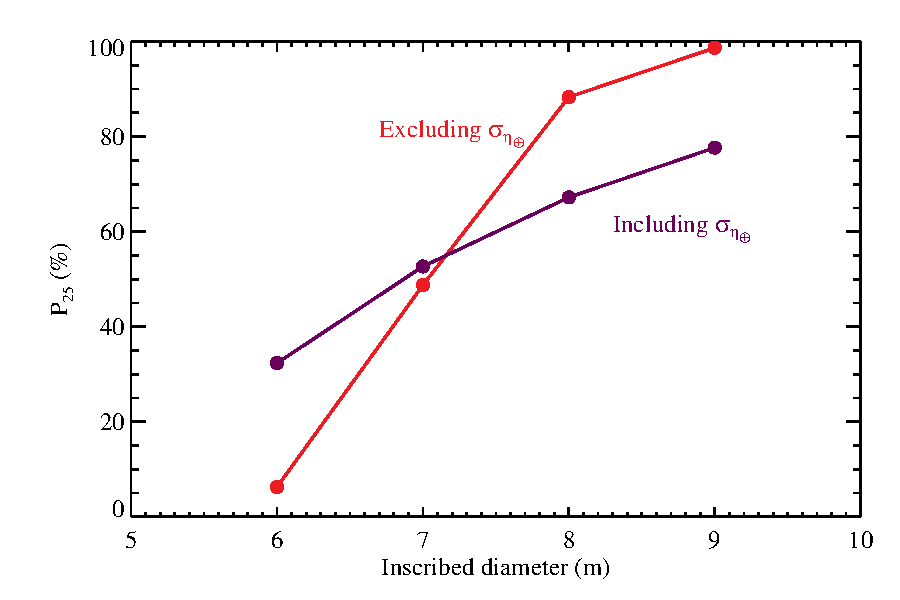
\includegraphics[width=\linewidth]{../ComparePublishedFigures/reference/starkFigure15.pdf}\end{minipage}\hfill
\begin{minipage}{0.48\textwidth}\centering\textbf{This model}\\[2pt]
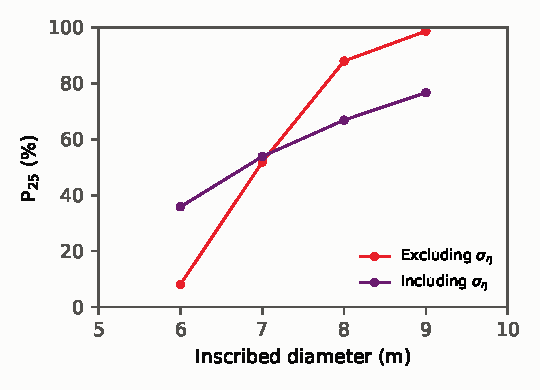
\includegraphics[width=\linewidth]{figMatchStarkFig15.pdf}\end{minipage}
\caption{$P_{25}$, the probability of at least 25 candidates, against inscribed diameter (6/7/8/9\,m). Including the uncertainty in $\eta_\oplus$: published 32/53/67/78\%, model 35 / 53 / 66 / 76\%. Excluding it: published 6/49/89/99.5\%, model 6 / 48 / 86 / 98\%.}
\label{fig:pair15}
\end{figure}

\begin{figure}[htbp]
\centering
\begin{minipage}{0.48\textwidth}\centering\textbf{Stark et al.\ (2024) Fig.~25}\\[2pt]
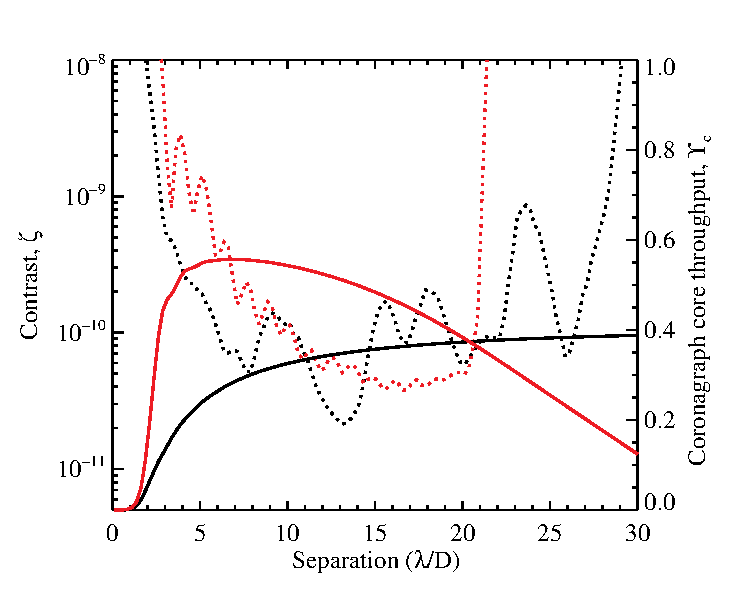
\includegraphics[width=\linewidth]{../ComparePublishedFigures/reference/starkFigure25.pdf}\end{minipage}\hfill
\begin{minipage}{0.48\textwidth}\centering\textbf{This model}\\[2pt]
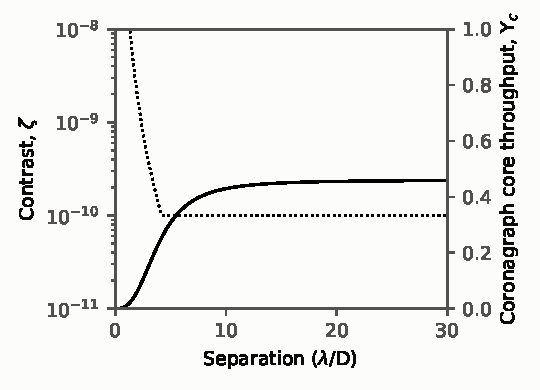
\includegraphics[width=\linewidth]{figMatchStarkFig25.pdf}\end{minipage}
\caption{DMVC6 raw contrast (dotted) and core throughput (solid) against separation in circumscribed $\lambda/D$. The model curves are the digitized published ones, evaluated exactly as the count rates use them, so this pair checks the digitization, not the model. The model's contrast is drawn with the $10^{-10}$ floor applied, as the exposure-time calculation uses it; the published curve is the raw simulation. The published figure also shows the PIAA-FPM2.5 coronagraph (red), which is not used here.}
\label{fig:pair25}
\end{figure}


%======================================================================
\section{Ledger of hypotheses tested}
\label{app:ledger}
%======================================================================

The reproduction proceeded by forming hypotheses about the source of each disagreement and testing
them. We record the full ledger because the distinction between a hypothesis rejected on evidence
and a real defect that turned out not to explain the symptom is load-bearing: a defect can be
genuine, worth fixing, and irrelevant to the symptom that led to it. Four separate times an
apparent agreement rested on two errors that cancelled, which is the reason this paper reports
conditional agreement rather than agreement.

\begin{table}[htbp]
\centering
\scriptsize
\begin{tabular}{p{4.6cm}p{2.6cm}p{8.0cm}}
\toprule
\textbf{Hypothesis} & \textbf{Outcome} & \textbf{Evidence} \\
\midrule
Missing revisits & \textbf{Real, a cause} & Single-visit only; modeling up to six visits raised the uncalibrated yield 1.7$\times$. \\
Characterization-time statistic & \textbf{Real, a cause} & A median over all detectable planets, where the budget needs a mean over those counted; $D^{1.11} \to D^{1.88}$. \\
Over-cap characterization charged & \textbf{Real, a cause} & 15\,000 days charged at 20\,pc for an observation never attempted. \\
Reconstructed target catalog & \textbf{Real, a cause} & HPIC was reachable; the Gaia stand-in lacked 26--34\% of distant FGK dwarfs and ran hot. \\
Coronagraph aperture convention & \textbf{Real, the cause} & Curves are in circumscribed $\lambda/D$; the IWA sat 19\% too far out. Yield 14.7 $\to$ 18.7. \\
Collecting area as inscribed circle & \textbf{Real, partial} & Charged the Lyot discard twice. \\
Characterization at detection phase & \textbf{Real, a cause} & Stark (2019) Sec.~5: the orbit is known, so ``the phase of the planet could be optimized. \\
Characterization budget under albedo draw & \textbf{Real, a cause} & Stark (2024) Sec.~3.2 fixes it at $A_G = 0.2$; albedo penalty 0.050 $\to$ 0.087. \\
Constant $T_{\rm sky}$ & \textbf{Real, the cause of $\kappa$} & Stark (2019) Eqs.~5--6 make it a map; with it the uncalibrated yield is 20.92 and $\kappa$ falls 1.62 $\to$ 0.987. Characterization times barely move. \\
Fitted throughput factor $\kappa$ & \textbf{Real, removed} & 22.5 is an output of AYO; once refitted, $\kappa$ turned every tested lever into a near-uniform $1.0 \pm 0.05$ change in exposure times. \\
One exozodi draw & \textbf{Real, fixed} & Now 200 draws with the survey re-optimized per draw; exozodi penalty 12.2\% (Stark 11.1\%). \\
Split $\kappa$ (detection vs spectra) & Rejected & A scalar on spectra cannot change the 6/9\,m characterization-time ratio. \\
Exozodi drawn during calibration & \textbf{Real, a cause} & $\kappa$ fitted to a drawn-exozodi yield cancels the exozodi penalty. \\
Lognormal exozodi stand-in & \textbf{Real, a cause} & 0.2\% of stars above 100 zodis vs 21\% in HOSTS; penalty 0.7\% $\to$ 12.2\%. \\
Pinned LBTI stars omitted & \textbf{Real, partial} & Worth at most 0.47 EEC here. \\
$\eta_\oplus$ interval read as 86\% & \textbf{Real, the cause of the shape} & Fig.~10 requires $\ln$-width $\sim$0.8; distance 0.142 $\to$ 0.024. \\
Published mode ill-determined & \textbf{Rejected} & Stark's 498 runs carry 1000 planet draws each; an earlier bootstrap resampled only 498 yields. \\
Fig.~4 mean compared with the wrong yield & \textbf{Real, not the cause} & Fig.~4 is sampling only at $A_G = 0.2$; the check is independent now that nothing is fitted. \\
$T_{\rm sky}$ missing; exozodi law & \textbf{Real, not the cause} & Backgrounds 1.48$\times$ too bright; constant-surface-brightness law. Together 1\%. \\
Contrast floor inside the knee & \textbf{Real, not the cause} & Floor applied universally. \\
Noise-floor screen & \textbf{Real, not the cause} & Admitted nothing above 4.6\,$L_\odot$. \\
Screening cap, uniform bias, bandpass choice & Rejected & 1.3\%, destroys 7--9\,m, 0.01. \\
Two detections for orbits & Rejected & Shifts the curve, does not narrow it. \\
Equal-slope allocation & Rejected & 0.00\% from an exact optimum. \\
Blackbody stellar flux & Rejected & +0.019\,mag against measured $V$. \\
Re-derived exposures at the drawn albedo & Replaced & Stark's per-visit test, both bounds, is adopted; it contributes 0.9\% of the Fig.~10 disagreement and gives a penalty of 3.6\% (published 12\%). \\
Noise floor, CIC definition, IFS pixels, ordering, dust color & Rejected & Sec.~\ref{sec:char}. \\
\bottomrule
\end{tabular}
\caption{The ledger. The traps that recur --- compensating errors, comparing against the wrong
published curve, biased diagnostic sub-samples, and read-off values --- are documented in
\texttt{doc/handoffToNextAgent.md}.}
\end{table}

%======================================================================
\section{Every contributing star}
\label{app:stars}
%======================================================================

{\scriptsize
\setlength{\tabcolsep}{3pt}
\begin{longtable}{llrrrrrrrrr}
\toprule
\textbf{Star} & \textbf{SpT} & \textbf{$d$ (pc)} & \textbf{$L$ ($L_\odot$)} & \textbf{Earth zone (mas)} & \textbf{classic HZ (mas)} & \textbf{$C_{\rm HZ}$} & \textbf{$C_{\rm EZ}$} & \textbf{$N_{\rm HZ}$} & \textbf{$N_{\rm EZ}$} & \textbf{ratio} \\
\midrule
\endhead
alf Cen B & K1V & 1.35 & 0.552 & 529--661 & 524--921 & 0.49 & 0.65 & 0.250 & 0.052 & 0.21 \\
HD  95735 & M2+V & 2.55 & 0.0239 & 58--73 & 58--101 & 0.99 & 1.00 & 0.249 & 0.052 & 0.21 \\
tau Cet & G8V & 3.65 & 0.52 & 189--237 & 188--330 & 0.98 & 1.00 & 0.248 & 0.052 & 0.21 \\
eps Ind & K5V & 3.64 & 0.222 & 124--155 & 123--216 & 0.98 & 1.00 & 0.247 & 0.052 & 0.21 \\
61 Cyg A & K5V & 3.50 & 0.158 & 109--136 & 108--190 & 0.98 & 1.00 & 0.247 & 0.052 & 0.21 \\
61 Cyg B & K7V & 3.50 & 0.104 & 89--111 & 88--154 & 0.98 & 1.00 & 0.246 & 0.052 & 0.21 \\
HD 217987 & M2V & 3.29 & 0.0413 & 59--74 & 59--103 & 0.97 & 1.00 & 0.245 & 0.052 & 0.21 \\
V* AX Mic & M1V & 3.97 & 0.105 & 78--98 & 77--136 & 0.96 & 1.00 & 0.239 & 0.051 & 0.21 \\
70 Oph A & K0V & 5.11 & 0.514 & 135--168 & 133--234 & 0.95 & 1.00 & 0.237 & 0.051 & 0.22 \\
del Equ & F7(V)+G & 4.51 & 0.265 & 110--137 & 108--191 & 0.95 & 1.00 & 0.236 & 0.052 & 0.22 \\
omi02 Eri & K0V & 5.01 & 0.428 & 125--157 & 124--218 & 0.95 & 1.00 & 0.236 & 0.052 & 0.22 \\
eps Eri & K2V & 3.22 & 0.342 & 174--218 & 173--303 & 0.96 & 1.00 & 0.236 & 0.051 & 0.22 \\
70 Oph B & K4V & 5.10 & 0.162 & 76--95 & 75--132 & 0.92 & 0.99 & 0.229 & 0.051 & 0.22 \\
e Eri & G6V & 6.04 & 0.663 & 129--162 & 128--225 & 0.91 & 0.99 & 0.223 & 0.051 & 0.23 \\
36 Oph & K2V+K1V & 5.95 & 0.334 & 93--117 & 92--162 & 0.90 & 0.97 & 0.222 & 0.050 & 0.22 \\
sig Dra & K0V & 5.76 & 0.433 & 110--137 & 108--191 & 0.89 & 0.98 & 0.221 & 0.051 & 0.23 \\
IRAS 20079-3614 &  & 6.01 & 0.26 & 81--102 & 81--142 & 0.88 & 0.94 & 0.221 & 0.049 & 0.22 \\
HD  88230 & K6VeFe- & 4.87 & 0.117 & 68--84 & 67--118 & 0.89 & 0.97 & 0.220 & 0.050 & 0.23 \\
HD 131977 & K4V & 5.89 & 0.223 & 77--96 & 76--134 & 0.87 & 0.94 & 0.218 & 0.049 & 0.22 \\
V* GX And & M2V & 3.56 & 0.0239 & 42--52 & 41--72 & 0.86 & 0.88 & 0.217 & 0.046 & 0.21 \\
36 Oph B & K1V & 5.95 & 0.331 & 93--116 & 92--162 & 0.87 & 0.96 & 0.216 & 0.049 & 0.23 \\
eta Cas & F9V & 5.92 & 1.27 & 182--228 & 181--317 & 0.88 & 0.99 & 0.214 & 0.051 & 0.24 \\
ksi Boo & G7Ve+K5 & 6.75 & 0.554 & 106--132 & 105--184 & 0.86 & 0.92 & 0.213 & 0.048 & 0.22 \\
HD 219134 & K3V & 6.54 & 0.29 & 79--99 & 78--137 & 0.84 & 0.89 & 0.211 & 0.046 & 0.22 \\
del Pav & G8IV & 6.10 & 1.25 & 176--220 & 174--306 & 0.87 & 0.99 & 0.210 & 0.050 & 0.24 \\
V* V2215 Oph & K5V & 5.95 & 0.158 & 64--80 & 63--111 & 0.84 & 0.87 & 0.210 & 0.045 & 0.22 \\
107 Psc & K1V & 7.64 & 0.458 & 85--106 & 84--148 & 0.83 & 0.87 & 0.205 & 0.045 & 0.22 \\
mu. Cas & G5Vb & 7.68 & 0.479 & 87--108 & 86--151 & 0.79 & 0.82 & 0.194 & 0.042 & 0.22 \\
HD 173739 & M3V & 3.52 & 0.016 & 35--43 & 34--60 & 0.76 & 0.69 & 0.193 & 0.036 & 0.19 \\
61 Vir & G6.5V & 8.53 & 0.841 & 103--129 & 102--179 & 0.78 & 0.84 & 0.192 & 0.043 & 0.22 \\
HD  16160 & K3V & 7.23 & 0.282 & 71--88 & 70--123 & 0.77 & 0.80 & 0.191 & 0.041 & 0.22 \\
bet CVn & G0V & 8.47 & 1.22 & 125--156 & 124--218 & 0.78 & 0.85 & 0.190 & 0.043 & 0.23 \\
HD 156384 & K3V+K5V & 6.97 & 0.192 & 60--76 & 60--105 & 0.74 & 0.77 & 0.186 & 0.040 & 0.21 \\
HD   4628 & K2.5V & 7.43 & 0.3 & 71--88 & 70--123 & 0.73 & 0.75 & 0.181 & 0.039 & 0.22 \\
V* TW PsA & K4Ve & 7.60 & 0.196 & 56--70 & 55--97 & 0.72 & 0.78 & 0.180 & 0.041 & 0.23 \\
p Eri A & K2V & 8.19 & 0.345 & 69--86 & 68--120 & 0.72 & 0.77 & 0.179 & 0.040 & 0.22 \\
chi01 Ori & G0V & 8.70 & 1.11 & 116--145 & 115--202 & 0.73 & 0.79 & 0.177 & 0.041 & 0.23 \\
p Eri B & K2V & 8.20 & 0.305 & 65--81 & 64--112 & 0.71 & 0.76 & 0.177 & 0.039 & 0.22 \\
ksi Boo B & K5Ve & 6.75 & 0.127 & 51--63 & 50--88 & 0.70 & 0.74 & 0.177 & 0.038 & 0.22 \\
HD 192310 & K2+V & 8.81 & 0.405 & 69--87 & 69--121 & 0.71 & 0.79 & 0.175 & 0.041 & 0.23 \\
ksi UMa & F8.5:V+ & 8.73 & 0.796 & 98--123 & 97--171 & 0.71 & 0.77 & 0.175 & 0.039 & 0.22 \\
ksi UMa A & F8.5:V & 8.73 & 1.26 & 123--154 & 122--214 & 0.72 & 0.80 & 0.173 & 0.040 & 0.23 \\
zet Tuc & F9.5V & 8.61 & 1.28 & 126--158 & 125--220 & 0.70 & 0.76 & 0.171 & 0.039 & 0.23 \\
41 Ara & G9V & 8.79 & 0.461 & 74--93 & 73--129 & 0.69 & 0.75 & 0.169 & 0.039 & 0.23 \\
HD 131976 & M1.5V & 5.90 & 0.0723 & 44--55 & 43--76 & 0.67 & 0.67 & 0.169 & 0.035 & 0.21 \\
kap01 Cet & G5V & 9.27 & 0.881 & 97--122 & 96--169 & 0.69 & 0.76 & 0.168 & 0.039 & 0.23 \\
HD 102365 & G2V & 9.32 & 0.849 & 95--119 & 94--165 & 0.68 & 0.77 & 0.166 & 0.040 & 0.24 \\
bet Com & F9.5V & 9.20 & 1.42 & 124--155 & 123--216 & 0.69 & 0.76 & 0.165 & 0.039 & 0.23 \\
alf Cen A & G2V & 1.35 & 1.66 & 918--1147 & 908--1596 & 0.18 & 0.24 & 0.164 & 0.030 & 0.18 \\
61 UMa & G8V & 9.57 & 0.625 & 79--99 & 78--138 & 0.67 & 0.76 & 0.163 & 0.039 & 0.24 \\
chi Dra & F7V & 8.30 & 2.19 & 171--214 & 170--298 & 0.69 & 0.83 & 0.163 & 0.041 & 0.25 \\
gam Pav & F9VFe-1 & 9.26 & 1.46 & 125--157 & 124--218 & 0.67 & 0.76 & 0.160 & 0.039 & 0.24 \\
pi.03 Ori & F6V & 8.02 & 2.85 & 202--253 & 200--352 & 0.68 & 0.86 & 0.157 & 0.043 & 0.27 \\
mu.01 Her & G5IV & 8.33 & 2.68 & 188--235 & 186--328 & 0.67 & 0.86 & 0.156 & 0.042 & 0.27 \\
alf Men & G7V & 10.21 & 0.866 & 87--109 & 87--152 & 0.64 & 0.74 & 0.154 & 0.038 & 0.25 \\
gam Lep & F6V & 8.90 & 2.36 & 166--207 & 164--288 & 0.66 & 0.79 & 0.154 & 0.040 & 0.26 \\
bet Hyi & G0V & 7.48 & 3.57 & 243--303 & 240--422 & 0.64 & 0.92 & 0.152 & 0.044 & 0.29 \\
del Tri & G0.5VFe & 10.91 & 1.21 & 97--121 & 96--168 & 0.63 & 0.80 & 0.152 & 0.041 & 0.27 \\
HD  10780 & K0V & 10.04 & 0.536 & 70--88 & 69--122 & 0.60 & 0.73 & 0.147 & 0.038 & 0.26 \\
HD  32147 & K3+V & 8.84 & 0.29 & 58--73 & 58--102 & 0.59 & 0.67 & 0.146 & 0.035 & 0.24 \\
HD  79210 & K7V & 6.33 & 0.0813 & 43--54 & 43--75 & 0.57 & 0.52 & 0.144 & 0.027 & 0.19 \\
tet Per & F8V & 11.14 & 2.32 & 131--164 & 130--228 & 0.61 & 0.82 & 0.142 & 0.041 & 0.29 \\
12 Oph & K1V & 9.89 & 0.46 & 66--82 & 65--114 & 0.58 & 0.70 & 0.142 & 0.036 & 0.26 \\
iot Per & G0V & 10.57 & 2.26 & 136--171 & 135--237 & 0.61 & 0.78 & 0.141 & 0.039 & 0.28 \\
V* AK Lep & K3 & 8.89 & 0.279 & 57--71 & 56--99 & 0.56 & 0.63 & 0.139 & 0.033 & 0.24 \\
del Eri & K0+IV & 9.09 & 3.29 & 192--240 & 190--333 & 0.59 & 0.82 & 0.136 & 0.040 & 0.29 \\
HD  36395 & M1.5Ve & 5.70 & 0.0594 & 41--51 & 41--71 & 0.53 & 0.47 & 0.134 & 0.024 & 0.18 \\
11 LMi & G8Va & 11.23 & 0.801 & 77--96 & 76--133 & 0.53 & 0.70 & 0.128 & 0.036 & 0.28 \\
zet Dor & F9VFe-0 & 11.69 & 1.48 & 100--125 & 99--174 & 0.53 & 0.72 & 0.125 & 0.037 & 0.29 \\
lam Ser & G0-V & 11.90 & 2.03 & 115--144 & 114--200 & 0.54 & 0.73 & 0.125 & 0.037 & 0.30 \\
zet TrA & F9V & 12.07 & 1.34 & 92--115 & 91--160 & 0.51 & 0.71 & 0.121 & 0.036 & 0.30 \\
20 Crt & K0V & 9.56 & 0.371 & 61--77 & 61--106 & 0.48 & 0.57 & 0.120 & 0.029 & 0.24 \\
lam Aur & G1.5IV- & 12.56 & 1.78 & 102--128 & 101--178 & 0.50 & 0.72 & 0.117 & 0.036 & 0.31 \\
gam Ser & F6V & 11.16 & 2.96 & 148--185 & 147--258 & 0.50 & 0.71 & 0.114 & 0.034 & 0.30 \\
HD  50281 & K3.5V & 8.74 & 0.219 & 51--64 & 51--89 & 0.46 & 0.41 & 0.114 & 0.021 & 0.19 \\
HD  42581 & M1V & 5.76 & 0.0515 & 38--47 & 37--66 & 0.44 & 0.19 & 0.111 & 0.010 & 0.09 \\
HD  79211 & M0V & 6.33 & 0.0707 & 40--50 & 40--70 & 0.44 & 0.24 & 0.111 & 0.013 & 0.11 \\
zet02 Ret & G1V & 12.04 & 1.02 & 80--100 & 80--140 & 0.46 & 0.63 & 0.110 & 0.032 & 0.29 \\
bet Vir & F9V & 11.00 & 3.69 & 168--209 & 166--292 & 0.48 & 0.74 & 0.108 & 0.035 & 0.33 \\
iot Peg & F5V & 11.90 & 3.57 & 152--191 & 151--265 & 0.48 & 0.75 & 0.108 & 0.035 & 0.33 \\
36 UMa & F8V & 12.94 & 1.63 & 95--118 & 94--165 & 0.46 & 0.66 & 0.107 & 0.034 & 0.31 \\
zet01 Ret & G2.5VHd & 12.04 & 0.795 & 71--89 & 70--124 & 0.44 & 0.53 & 0.106 & 0.027 & 0.26 \\
HD  17925 & K1V & 10.36 & 0.401 & 59--73 & 58--102 & 0.41 & 0.38 & 0.100 & 0.019 & 0.19 \\
HD 191849 & M0V & 6.16 & 0.0616 & 39--48 & 38--67 & 0.38 & 0.15 & 0.095 & 0.008 & 0.08 \\
54 Psc & K0.5V & 11.10 & 0.529 & 63--79 & 62--109 & 0.38 & 0.39 & 0.092 & 0.020 & 0.22 \\
ups And & F9V & 13.47 & 3.38 & 131--164 & 130--228 & 0.41 & 0.67 & 0.090 & 0.032 & 0.35 \\
HD 157881 & K7V & 7.71 & 0.123 & 44--55 & 43--76 & 0.35 & 0.16 & 0.087 & 0.008 & 0.09 \\
HD 103095 & K1V\_Fe- & 9.17 & 0.235 & 51--63 & 50--88 & 0.34 & 0.23 & 0.085 & 0.012 & 0.14 \\
10 Tau & F9IV-V & 13.92 & 3.16 & 123--153 & 121--213 & 0.37 & 0.61 & 0.084 & 0.029 & 0.35 \\
47 UMa & G1-VFe- & 13.88 & 1.6 & 87--109 & 86--152 & 0.36 & 0.50 & 0.084 & 0.025 & 0.30 \\
gam Vir & F1-F2V & 12.02 & 4.55 & 170--213 & 169--296 & 0.38 & 0.65 & 0.083 & 0.029 & 0.36 \\
alf CMi & F5IV-V+ & 3.50 & 7.21 & 737--921 & 729--1282 & 0.15 & 0.30 & 0.080 & 0.028 & 0.36 \\
tau01 Eri & F7V & 14.27 & 2.67 & 110--137 & 109--191 & 0.34 & 0.53 & 0.080 & 0.026 & 0.33 \\
iot Psc & F7V & 13.66 & 3.39 & 129--162 & 128--225 & 0.35 & 0.59 & 0.079 & 0.028 & 0.36 \\
HD 119850 & M2V & 5.43 & 0.0397 & 35--44 & 35--61 & 0.30 & 0.06 & 0.076 & 0.003 & 0.04 \\
alf For & F6V & 14.00 & 4.28 & 142--177 & 140--247 & 0.35 & 0.60 & 0.076 & 0.027 & 0.36 \\
HD 104304 & G8IV & 12.76 & 0.892 & 71--89 & 70--124 & 0.32 & 0.34 & 0.076 & 0.017 & 0.23 \\
HD 223778 & K3V & 10.89 & 0.399 & 56--70 & 55--97 & 0.30 & 0.19 & 0.074 & 0.010 & 0.13 \\
eta Cas B & K7Ve & 5.93 & 0.0513 & 37--46 & 36--64 & 0.29 & 0.04 & 0.074 & 0.002 & 0.03 \\
alf Com & F5V+F6V & 14.32 & 3 & 116--145 & 115--202 & 0.32 & 0.51 & 0.072 & 0.025 & 0.35 \\
HD 147513 & G5V & 12.89 & 0.998 & 74--93 & 74--129 & 0.29 & 0.35 & 0.071 & 0.018 & 0.25 \\
V* DE Boo & K0.5V & 11.63 & 0.541 & 61--76 & 60--106 & 0.29 & 0.21 & 0.070 & 0.011 & 0.15 \\
HD  13445 & K1.5V & 10.76 & 0.406 & 57--71 & 56--99 & 0.28 & 0.20 & 0.070 & 0.010 & 0.14 \\
gam Vir B & F0mF2V & 12.74 & 5.27 & 173--216 & 171--301 & 0.32 & 0.56 & 0.069 & 0.025 & 0.37 \\
HD 122064 & K3V & 10.06 & 0.291 & 51--64 & 51--89 & 0.28 & 0.12 & 0.068 & 0.006 & 0.09 \\
58 Eri & G2.5IV- & 13.23 & 0.966 & 71--89 & 71--124 & 0.28 & 0.26 & 0.066 & 0.013 & 0.20 \\
psi Cap & F5V & 14.63 & 3.72 & 127--158 & 125--220 & 0.29 & 0.48 & 0.064 & 0.023 & 0.35 \\
85 Peg & G5VbFe- & 12.32 & 0.674 & 64--80 & 63--111 & 0.26 & 0.21 & 0.064 & 0.011 & 0.17 \\
111 Tau & F8V & 14.57 & 1.78 & 88--110 & 87--153 & 0.27 & 0.35 & 0.062 & 0.017 & 0.28 \\
HD  10307 & G1V & 14.67 & 1.89 & 90--112 & 89--157 & 0.26 & 0.37 & 0.061 & 0.019 & 0.31 \\
26 Dra & F9V+K3V & 14.43 & 1.48 & 81--101 & 80--141 & 0.26 & 0.31 & 0.060 & 0.016 & 0.26 \\
HD 211415 & G0V & 14.06 & 1.17 & 74--92 & 73--129 & 0.25 & 0.23 & 0.059 & 0.012 & 0.20 \\
chi Her & F8VFe-2 & 15.90 & 3.16 & 107--134 & 106--187 & 0.26 & 0.40 & 0.058 & 0.020 & 0.34 \\
zet Her & G0IV & 10.80 & 7.26 & 240--300 & 237--417 & 0.26 & 0.49 & 0.055 & 0.020 & 0.36 \\
nu. Phe & F9VFe+0 & 15.25 & 2.03 & 90--112 & 89--156 & 0.24 & 0.30 & 0.055 & 0.015 & 0.28 \\
b Aql & G7IVHde & 14.91 & 1.7 & 84--105 & 83--146 & 0.23 & 0.28 & 0.053 & 0.014 & 0.27 \\
alf Crv & F1V & 14.97 & 4.34 & 134--167 & 132--232 & 0.23 & 0.39 & 0.051 & 0.018 & 0.35 \\
HD  84117 & F9V & 14.95 & 2.01 & 91--114 & 90--159 & 0.22 & 0.30 & 0.051 & 0.015 & 0.29 \\
h Dra & F8V & 15.33 & 2.28 & 95--118 & 94--164 & 0.22 & 0.29 & 0.051 & 0.015 & 0.29 \\
tau Boo & F7IV-V & 15.60 & 3.18 & 110--137 & 109--191 & 0.23 & 0.33 & 0.050 & 0.016 & 0.32 \\
sig Boo & F4VkF2m & 15.75 & 3.22 & 109--137 & 108--190 & 0.21 & 0.29 & 0.047 & 0.014 & 0.30 \\
eta Lep & F2V & 14.95 & 5.66 & 153--191 & 151--266 & 0.22 & 0.37 & 0.047 & 0.016 & 0.35 \\
171 Pup & F9V & 15.27 & 1.57 & 79--99 & 78--137 & 0.19 & 0.19 & 0.046 & 0.010 & 0.21 \\
m Tau & G4V & 15.91 & 2.41 & 94--117 & 93--163 & 0.20 & 0.27 & 0.045 & 0.013 & 0.29 \\
18 Sco & G2Va & 14.13 & 1.1 & 71--89 & 70--124 & 0.19 & 0.14 & 0.045 & 0.007 & 0.16 \\
mu. Ara & G3IV-V & 15.60 & 1.9 & 85--106 & 84--148 & 0.20 & 0.22 & 0.044 & 0.011 & 0.25 \\
20 LMi & G3VaHde & 14.92 & 1.37 & 75--94 & 75--131 & 0.18 & 0.15 & 0.043 & 0.008 & 0.18 \\
b Her & F6V & 15.76 & 2.02 & 87--108 & 86--151 & 0.19 & 0.21 & 0.043 & 0.010 & 0.24 \\
HD 176051 & F9V+K1V & 14.89 & 1.42 & 77--96 & 76--134 & 0.18 & 0.16 & 0.043 & 0.008 & 0.19 \\
HD  69830 & G8:V & 12.58 & 0.609 & 60--74 & 59--104 & 0.18 & 0.05 & 0.043 & 0.002 & 0.06 \\
HD 160346 & K3-V & 10.71 & 0.32 & 51--63 & 50--88 & 0.17 & 0.02 & 0.042 & 0.001 & 0.03 \\
ksi Peg & F6V & 16.39 & 4.76 & 128--160 & 126--222 & 0.19 & 0.30 & 0.042 & 0.013 & 0.32 \\
rho01 Cnc & K0IV-V & 12.58 & 0.635 & 61--76 & 60--106 & 0.17 & 0.06 & 0.041 & 0.003 & 0.07 \\
HD 166620 & K2V & 11.09 & 0.363 & 52--65 & 52--91 & 0.16 & 0.02 & 0.040 & 0.001 & 0.03 \\
tet UMa & F7V & 13.53 & 7.9 & 199--249 & 197--347 & 0.18 & 0.35 & 0.037 & 0.013 & 0.36 \\
eta Boo & G0IV & 11.34 & 8.79 & 251--314 & 248--437 & 0.16 & 0.33 & 0.035 & 0.013 & 0.37 \\
bet TrA & F1V & 12.42 & 8.71 & 228--285 & 226--397 & 0.16 & 0.30 & 0.033 & 0.012 & 0.35 \\
I Car & F3V & 16.28 & 5.25 & 135--169 & 134--235 & 0.14 & 0.22 & 0.031 & 0.010 & 0.33 \\
HD 172051 & G6V & 13.02 & 0.682 & 61--76 & 60--106 & 0.12 & 0.02 & 0.029 & 0.001 & 0.03 \\
i Boo & G0Vn & 12.95 & 0.639 & 59--74 & 59--103 & 0.12 & 0.01 & 0.028 & 0.000 & 0.02 \\
gam CrA A & F8V & 17.03 & 2.47 & 89--111 & 88--154 & 0.13 & 0.12 & 0.028 & 0.006 & 0.20 \\
tau01 Hya & F5V & 18.24 & 4.05 & 106--132 & 105--184 & 0.13 & 0.19 & 0.028 & 0.008 & 0.30 \\
HD   3443 & K1V+G & 15.53 & 1.32 & 71--89 & 70--123 & 0.12 & 0.05 & 0.027 & 0.002 & 0.08 \\
9 Pup & G0V & 16.67 & 1.95 & 80--101 & 80--140 & 0.12 & 0.07 & 0.026 & 0.004 & 0.14 \\
HD 188088 & K3VaCN1 & 14.14 & 0.803 & 61--76 & 60--106 & 0.11 & 0.01 & 0.026 & 0.000 & 0.02 \\
nu.02 Lup & G3/5V & 14.74 & 1.04 & 66--83 & 66--115 & 0.11 & 0.02 & 0.026 & 0.001 & 0.03 \\
pi.01 UMa & G0.5V & 14.43 & 0.972 & 66--82 & 65--114 & 0.11 & 0.01 & 0.026 & 0.001 & 0.03 \\
phi02 Cet & F7V & 15.92 & 1.79 & 81--101 & 80--140 & 0.11 & 0.07 & 0.025 & 0.004 & 0.15 \\
gam CrA & F8V+F8V & 17.89 & 4.8 & 118--147 & 116--204 & 0.11 & 0.13 & 0.023 & 0.006 & 0.26 \\
HD  37394 & K1 & 12.26 & 0.477 & 54--68 & 53--94 & 0.09 & 0.00 & 0.023 & 0.000 & 0.00 \\
HD 115404 & K2V & 10.98 & 0.302 & 48--60 & 48--84 & 0.09 & 0.00 & 0.022 & 0.000 & 0.00 \\
del Aql & F1IV-V( & 15.37 & 8.26 & 179--224 & 178--312 & 0.11 & 0.20 & 0.022 & 0.008 & 0.35 \\
70 Vir & G4Va & 18.09 & 3.1 & 93--117 & 93--163 & 0.10 & 0.10 & 0.022 & 0.005 & 0.22 \\
51 Peg & G2IV & 15.51 & 1.38 & 73--91 & 72--126 & 0.09 & 0.03 & 0.021 & 0.002 & 0.07 \\
g Lup & F3/5V & 17.39 & 3.33 & 101--126 & 100--175 & 0.10 & 0.09 & 0.021 & 0.004 & 0.20 \\
58 Oph & F5V & 17.17 & 2.72 & 92--115 & 91--160 & 0.09 & 0.06 & 0.020 & 0.003 & 0.15 \\
HD  74576 & K3V & 11.19 & 0.318 & 48--60 & 48--84 & 0.08 & 0.00 & 0.020 & 0.000 & 0.00 \\
tau06 Eri & F5IV-V & 17.78 & 5.15 & 123--153 & 121--213 & 0.09 & 0.11 & 0.020 & 0.005 & 0.26 \\
psi05 Aur & F9V & 16.61 & 1.82 & 78--97 & 77--136 & 0.08 & 0.02 & 0.019 & 0.001 & 0.06 \\
ksi Oph & F2V & 17.50 & 4.35 & 114--143 & 113--199 & 0.09 & 0.09 & 0.018 & 0.004 & 0.22 \\
HD 103932 & K4+V & 10.17 & 0.212 & 43--54 & 43--76 & 0.07 & 0.00 & 0.018 & 0.000 & 0.00 \\
HD 217357 & K7+Vk & 8.23 & 0.101 & 37--46 & 37--64 & 0.06 & 0.00 & 0.015 & 0.000 & 0.00 \\
rho Gem & F1V & 17.83 & 5.44 & 126--157 & 124--218 & 0.07 & 0.08 & 0.015 & 0.003 & 0.22 \\
HD   5015 & F9V & 18.90 & 3.62 & 97--121 & 96--168 & 0.07 & 0.04 & 0.015 & 0.002 & 0.14 \\
HD 207129 & G2V & 15.55 & 1.21 & 68--85 & 67--118 & 0.06 & 0.00 & 0.014 & 0.000 & 0.01 \\
tet Cyg & F3+V & 18.42 & 4.27 & 108--135 & 107--187 & 0.07 & 0.05 & 0.014 & 0.002 & 0.17 \\
HD 114837 & F6VFe-0 & 18.23 & 2.99 & 91--114 & 90--158 & 0.06 & 0.03 & 0.013 & 0.002 & 0.12 \\
eta Crv & F2V & 18.24 & 4.77 & 115--144 & 114--200 & 0.06 & 0.05 & 0.012 & 0.002 & 0.17 \\
10 UMa & F3V+G5V & 18.79 & 6.73 & 132--166 & 131--230 & 0.06 & 0.07 & 0.012 & 0.003 & 0.23 \\
HD  32450 & K7V & 8.36 & 0.11 & 38--48 & 38--66 & 0.05 & 0.00 & 0.012 & 0.000 & 0.00 \\
e Vir & G0V & 17.57 & 2.19 & 81--101 & 80--141 & 0.05 & 0.01 & 0.010 & 0.000 & 0.03 \\
HD  72673 & K1V & 12.16 & 0.403 & 50--63 & 50--87 & 0.04 & 0.00 & 0.010 & 0.000 & 0.00 \\
\bottomrule
\end{longtable}
}

Stars with an expected yield of at least 0.01 EEC in either zone's survey, in order of
their classic-zone yield. Zone edges are angular separations in milliarcseconds; $C$ is the
completeness reached, averaged over exozodi draws; $N$ is the expected number of candidates. The
complete table is \texttt{TabulateEarthZones/earthZoneTable.csv}.

%======================================================================
\section*{References}
%======================================================================

\begin{description}\small
\item[{[bryson2021]}] Bryson, S., et al.\ 2021, AJ, 161, 36 (arXiv:2010.14812).
\item[{[savransky2016]}] Savransky, D., \& Garrett, D.\ 2016, JATIS, 2, 011006 (EXOSIMS).
\item[{[stark2014]}] Stark, C.~C., Roberge, A., Mandell, A., \& Robinson, T.~D.\ 2014, ApJ, 795, 122.
\item[{[stark2019]}] Stark, C.~C., et al.\ 2019, JATIS, 5, 024009 (arXiv:1904.11988).
\item[{[stark2024]}] Stark, C.~C., et al.\ 2024, JATIS (arXiv:2405.19418).
\item[{[stark2025]}] Stark, C.~C., et al.\ 2025, arXiv:2502.18556 (ETC benchmark).
\item[{[tuchow2024]}] Tuchow, N.~W., et al.\ 2024, the HWO Preliminary Input Catalog (HPIC).
\end{description}

\end{document}
